%% Augur -- AMT manuscript (Copernicus Publications, research article)
%% Class: official copernicus.cls (Copernicus LaTeX package 7.16, downloaded 2026-09-28).
%% Build:  latexmk -pdf main.tex        (or: pdflatex main; bibtex main; pdflatex main; pdflatex main)

\documentclass[amt, manuscript]{copernicus}

%% ---------------------------------------------------------------------------
%% Local macros (kept to a minimum so the source stays Copernicus-compatible)
%% ---------------------------------------------------------------------------
%% \fieldnum{...} marks every number taken from the field record (2026 deployment).
%% It prints its argument unchanged. Set \fielddrafttrue to colour them for proof-reading.
\newif\iffielddraft
\fielddraftfalse
% \fielddrafttrue
\newcommand{\fieldnum}[1]{\iffielddraft{\color{magenta}#1}\else#1\fi}
%% \strong{...} = bold emphasis carried over from the drafts (markdown **...**).
%% Copernicus copy-editing normally removes bold from running text; redefine to \emph if preferred.
\newcommand{\strong}[1]{\textbf{#1}}
\providecommand{\Sigmaup}{\Sigma}

\begin{document}

\title{Augur: an $\alpha$-domain variable-projection DOAS retrieval, and what its diagnostics reveal that standard fit reports do not}

% \Author[affil][email]{given_name}{surname}   -- author list to be completed by the authors
\Author[1][email-to-be-added]{First}{Author}
\Author[1]{Co}{Author}

\affil[1]{Gwangju Institute of Science and Technology (GIST), Gwangju, Republic of Korea}

\runningtitle{Augur: an $\alpha$-domain variable-projection DOAS retrieval}
\runningauthor{Author et al.}

\received{}
\pubdiscuss{}
\revised{}
\accepted{}
\published{}

\firstpage{1}

\maketitle

%% Abstract -- rewritten 2026-09-29 to the Copernicus length guideline (<= 250 words).
\begin{abstract}
A DOAS fit reports a residual, chi-square, uncertainty and convergence flag, read as a measure of retrieval
quality. We present Augur, an open retrieval that poses the fit in the extinction domain as a
separable nonlinear least-squares problem, solves it by variable projection and is configured by instrument and
campaign profiles. Its calibration references enter as data, so they can be perturbed, and the objective mapped, without
reprocessing a campaign. We use it on one field case, a
thermal-dissociation broadband cavity-enhanced absorption spectrometer \citep{Min_2016,Nam_2022} with two heated and one
ambient-temperature cavity, to measure two gaps between fit report and data.

The first is error the fit cannot see. For the alkyl nitrate product, leave-one-out perturbation of the zero-air,
reflectivity and etalon references gives, in the best-calibrated week, a structural uncertainty \fieldnum{1.28} to \fieldnum{2.29}
times the reported per-scan sigma, and a total \fieldnum{1.63} to \fieldnum{2.50} times, without enlarging the residual. The second is information the pipeline holds and
discards. The ambient-temperature channel's wavelength shift is not identifiable from ambient spectra, yet its fits
report convergence. A time-base error introduced by the pipeline, a reflectivity reference nine
hours out of alignment, displaced the product by \fieldnum{0.100}\,ppb while changing the residual and the reported uncertainty
by two parts in a thousand. A multiplicative scale error, evident only against a co-located reference analyser, is invisible to both.
We propose that each record carry its termination state, distance to the nearest calibration and reference
provenance, and release a synthetic benchmark for other implementations.
\end{abstract}


%% Sect. 1 -- from augur_AMT_§1 draft v1 (2026-09-21); research questions and restructuring 2026-09-29.
\introduction
\label{sec:1}

A DOAS retrieval returns more than a concentration. It returns a residual, a chi-square, a parameter covariance and a
convergence flag, and these travel with the concentration into averaging, filtering, trend fits and comparisons with
models and other instruments. They are read as a statement of trust: a small residual means the model described the spectrum, a converged flag
means the optimiser found the answer, and the reported 1$\sigma$ means the concentration is known that well. Each reading is conditional, and the conditions are not reported
alongside the numbers.

This paper asks two questions about that gap. First, how large are the errors that a fit report cannot see, when they
are measured by perturbing the calibration chain and re-running the retrieval? Second, what information does the
pipeline already hold, and discard, that would flag a failed retrieval? A third category emerges from the answers:
errors that neither the fit report nor any of the fields we propose can detect (Sect.~\ref{sec:6.5}).

The first question has a partial answer in the DOAS literature. The uncertainty a DOAS fit reports is the propagation
of the residual scatter through the linear system, and it is correct only if the residual is white and the forward
model complete. \citet{Stutz_1996} showed that structure in the residual inflates the true error beyond the reported
one, and the standard treatment \citep{Platt} sets out the conditions explicitly. Practitioners respond with rules of
thumb -- multiply the reported error by two, or by the ratio of the residual to the photon noise -- and with
sensitivity studies on the window, the polynomial order and the set of cross sections.

That literature examines the spectral fit. The quantities the fit treats as given -- the reference spectrum, the
mirror reflectivity, the instrument line shape -- are usually characterised separately, assigned a calibration
uncertainty and combined with the fit uncertainty at the end. For a cavity-enhanced instrument this is a strong
assumption. The reference and the reflectivity are time series, measured intermittently and interpolated to every
measurement, and the error they contribute to a record depends on where that record sits relative to the nearest
calibration. A campaign-mean calibration uncertainty, of the kind reported for the effective path length in earlier
instruments of the design used here \citep{Min_2016,Nam_2022}, does not describe it.

Intercomparisons and synthetic studies do not close this gap either. Intercomparisons such as CINDI-2
\citep{Kreher_2020} measure the spread between codes, which bounds implementation error and has standardised settings,
but codes that agree may share a mistake, and without a truth a disagreement cannot say which is right. Synthetic
studies supply that truth, but they test the fit for given references, which are correct by construction.

Treating the calibration chain as part of the retrieval divides the shortfalls of a fit report into two kinds with
different remedies. The first is what the fit cannot know: contributions that leave the residual unchanged, which have
to be measured by perturbing the retrieval and added to the budget. The second is what the pipeline already knows and
does not carry to the product: whether the optimiser stopped at a bound, whether the nearest reflectivity measurement
was fifteen minutes or eleven hours away, whether a quality gate rejected the neighbouring calibration blocks. This
information exists when the concentration is computed and is then discarded, although keeping it would turn a silent
failure into a flagged one.

We present Augur, an open retrieval built so that both kinds of question can be asked routinely. It poses the retrieval
in the extinction domain as a separable nonlinear least-squares problem and solves it by variable projection. The
layout of the raw data, the calibration flags and the fit configuration are read from instrument and campaign profiles
(Appendix~\ref{app:A}), so the same code runs other configurations. The diagnostics are demonstrated on one field case:
a thermal-dissociation broadband cavity-enhanced absorption spectrometer with two heated and one ambient-temperature
cavity, measuring NO$_2$, total peroxy nitrates and total alkyl nitrates over 53 days in 2026. Other configurations are
not evaluated here.

We verify the retrieval against synthetic truth and against an independent DOAS implementation. We then measure the
structural terms it cannot report, which together exceed the reported sigma by a factor of \fieldnum{1.6} to \fieldnum{2.5} in the
best-calibrated week, and map the identifiability of its nonlinear parameters. We also describe twelve days of
operational product built from a calibration reference that a later correction had made stale. That error was \fieldnum{1.44}
times the budget and moved the 300\,$^{\circ}$C channel's concentration by two reported standard deviations, while the residual
and the reported uncertainty changed by two parts in a thousand. We propose a small reporting convention whose distance
fields would have flagged it at the first reprocessing and whose provenance fields, once implemented, would name its
cause. Finally, we release a synthetic benchmark with which any DOAS implementation can measure the same quantities on
the same cases.

The evidence is one field case, one instrument over one campaign, which bounds what can be concluded about instruments
in general. Two results are intended to carry beyond it. The benchmark of Sect.~\ref{sec:3.4} contains no retrieval
code and no field data, so the measurements it supports do not depend on any implementation; its cross sections,
windows and wavelength grid are those of one instrument. The
reporting convention of Sect.~\ref{sec:6} asks for quantities that every implementation already computes, apart from the
build time and time convention of each reference, which must be recorded when the reference is built. Where a result
depends on this instrument, such as the magnitude of the reflectivity term or the behaviour of the cold channel, we say
so.

Figure~\ref{fig:1} previews the argument. Section~\ref{sec:2} sets out the retrieval and Sect.~\ref{sec:3} verifies it.
Sections~\ref{sec:4} and \ref{sec:5} take the two kinds of shortfall in turn, Sect.~\ref{sec:6} draws the reporting
convention out of them and names what it cannot reach, Sect.~\ref{sec:7} demonstrates it on the field case, and
Sect.~\ref{sec:8} concludes. Appendix~\ref{app:A} collects the instrument and retrieval configuration,
Appendix~\ref{app:B} the projected Jacobian and joint covariance, Appendix~\ref{app:C} the measurements on
calibration-block length, and Appendix~\ref{app:D} the choice of denominator for the budget ratio.

\begin{figure*}[t]
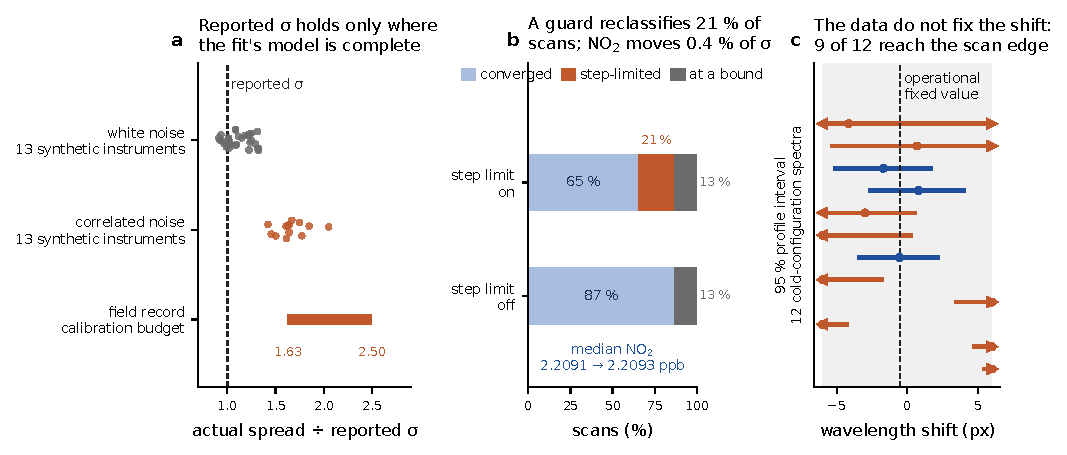
\includegraphics[width=\textwidth]{figures/fig01.pdf}
\caption{What a converged fit reports, and what the data support. \textbf{(a)} Spread of retrieved NO$_2$ over the
reported uncertainty. Grey: white noise, 30 cases over 13 synthetic instruments (line-shape width 0.5--2, window
0.7--1.3 and pixel dispersion 0.7--1.4 times nominal; signal-to-noise over a factor of 32; polynomial orders 2--6).
Orange: the same with AR(1) noise, $\rho = 0.5$. Bar: the field record, total uncertainty \fieldnum{1.63} (robust scale) to
\fieldnum{2.50} (standard deviation) times the fit-propagated $\sigma$ ($n = \fieldnum{8847}$ records of 60\,s). \textbf{(b)} Termination state
of \fieldnum{8446} operational scans, step limit on and off. \textbf{(c)} 95\,\% profile-likelihood
intervals of the cold-configuration shift for 12 spectra, scanned over $\pm6$\,px, with
$\mathrm{RSS}/\mathrm{RSS}_{\min} \le 1 + F_{0.95}(1, n-P)/(n-P)$, $n-P = 766$; arrows reach the scan edge;
dashed, the operational value, $-0.5$\,px.}
\label{fig:1}
\end{figure*}

%% Sect. 2 -- Sects. 2.1-2.6 from augur_AMT_§2 draft v1 (2026-09-19); Sect. 2.7 from the §2.9_3 draft (2026-09-21).
%% 2026-09-29 edit: implementation detail (QR, Eq. 7, Kaufman, relation to DOAS codes, scaling note, unused options)
%% moved to Appendix B5-B6.
\section{Retrieval formulation}
\label{sec:2}

\subsection{Forward model in the extinction domain}
\label{sec:2.1}

The cavity output is converted to an extinction coefficient before any spectral fitting
is attempted. For a sample spectrum $I(\lambda)$ and a reference spectrum
$I_0(\lambda)$ recorded with the cavity filled by zero air,
\begin{equation}
\alpha(\lambda) \;=\;
\Bigl[\underbrace{\tfrac{R_L\,(1-R(\lambda,t))}{d}}_{\textstyle \alpha_{\mathrm{mirror}}}
\;+\; R_L\,\alpha_{\mathrm{Ray}}(\lambda; T_0, P_0)\Bigr]
\frac{I_0(\lambda)-I(\lambda)}{I(\lambda)}
\;-\;\bigl[\alpha_{\mathrm{Ray}}(\lambda; T, P)-\alpha_{\mathrm{Ray}}(\lambda; T_0,P_0)\bigr],
\label{eq:1}
\end{equation}
where $R(\lambda,t)$ is the mirror reflectivity and $d$ the mirror separation. $R_L$ is the ratio of the full mirror
separation to the cavity length actually filled by the sample, excluding the purge-gas volumes at the mirrors, and
$\alpha_{\mathrm{Ray}}$ is the Rayleigh extinction at the temperature and pressure of the sample $(T,P)$ and of the
reference $(T_0,P_0)$. The first bracket converts a relative
intensity change into an absolute extinction; the second removes the Rayleigh difference between the two states. Light-level changes between reference and sample enter $\alpha$ directly, a sensitivity that the iterative
cavity-enhanced DOAS method of \citet{Horbanski_2019} removes.
In $\alpha$, unlike in optical density, the gas amounts enter linearly: the quantity to be fitted is a sum of
reference cross sections with concentration coefficients, a smooth background and the periodic structure the
optics impose.

\subsection{Separable structure}
\label{sec:2.2}

Let $p$ index the $n$ detector pixels of the fitting window and let
\begin{equation*}
x(p) \;=\; \frac{2\,(p-p_{\min})}{p_{\max}-p_{\min}} - 1 \;\in\; [-1,1].
\end{equation*}
The model for the measured extinction is
\begin{equation}
\alpha_{\text{model}}(p)\;=\;
\sum_{i=1}^{m} c_i\,\tau_i(T)\,\sigma_i\bigl(p_i'\bigr)
\;+\;\sum_{j=0}^{q} b_j\,T_j\bigl(x(p)\bigr)
\;+\; a_s \sin(f p) + a_c \cos(f p),
\label{eq:2}
\end{equation}
\begin{equation}
p_i' \;=\; (p-p_c)\,s_i + p_c + \delta_i ,
\label{eq:3}
\end{equation}
with $T_j$ the Chebyshev polynomial of the first kind, $p_c$ a fixed window centre,
and $\tau_i(T)=1+\kappa_i (T-T_{\mathrm{ref}})/100$ the temperature scaling of the
$i$-th cross section. Each reference carries its own wavelength shift $\delta_i$
(pixels) and squeeze $s_i$; in practice one gas is designated the anchor and the
companions are linked to it or fixed, which constrains $\theta$ without changing the structure.
The Chebyshev basis on $x\in[-1,1]$ keeps the background block well conditioned, where a monomial basis would
reach condition numbers that make the background coefficients meaningless and leak into the gas coefficients
through the shared normal equations. The etalon enters as a sine--cosine pair at fixed frequency: since
$A\sin(fp+\varphi)=A\cos\varphi\,\sin(fp)+A\sin\varphi\,\cos(fp)$, the pair $(a_s,a_c)$ spans the same model
space as $(A,\varphi)$ but is linear, so only the frequency $f$ is fixed a priori.

Collecting the $k=m+(q+1)+2$ basis vectors into a design matrix $\mathbf{A}(\theta)$
whose columns depend on the nonlinear vector $\theta=(\delta_i,s_i)$ only through
Eq.~(\ref{eq:3}), and writing $\mathbf{W}=\mathrm{diag}(w_1,\dots,w_n)$ for the pixel weights,
the problem is
\begin{equation}
\min_{\theta,\;\mathbf{c}}\;
\bigl\|\mathbf{W}\bigl(\mathbf{y}-\mathbf{A}(\theta)\,\mathbf{c}\bigr)\bigr\|_2^2,
\qquad \mathbf{y}=\alpha_{\text{meas}} .
\label{eq:4}
\end{equation}
This is a separable nonlinear least-squares problem in the sense of \citet{Golub_1973}:
$k$ linear parameters and, for the operational configuration, two to
six nonlinear ones.

\subsection{Variable projection with an analytic projected Jacobian}
\label{sec:2.3}

For any $\theta$ the inner problem is an ordinary linear least-squares problem, so
$\mathbf{c}$ need never be searched. Substituting the minimiser
$\hat{\mathbf{c}}(\theta)=\mathbf{A}^{+}\mathbf{y}$ leaves the projected residual
\begin{equation}
\mathbf{r}(\theta)\;=\;\bigl(\mathbf{I}-\mathbf{A}(\theta)\mathbf{A}(\theta)^{+}\bigr)\mathbf{y}
\;=\;\mathbf{P}^{\perp}_{\mathbf{A}(\theta)}\,\mathbf{y},
\label{eq:5}
\end{equation}
a function of $\theta$ alone, which we minimise with a bounded
Levenberg--Marquardt/trust-region solver. Its Jacobian is supplied analytically in the full Golub--Pereyra form,
\begin{equation}
\frac{\partial \mathbf{r}}{\partial \theta_k}
\;=\;-\Bigl[\;\underbrace{\mathbf{P}^{\perp}\mathbf{D}_k\,\hat{\mathbf{c}}}_{\text{projection term}}
\;+\;\underbrace{(\mathbf{A}^{+})^{\!\top}\mathbf{D}_k^{\top}\,\mathbf{r}}_{\text{second term}}\;\Bigr],
\qquad
\mathbf{D}_k=\frac{\partial \mathbf{A}}{\partial \theta_k}.
\label{eq:6}
\end{equation}
Retaining the second term makes Eq.~(\ref{eq:6}) the exact derivative rather than the \citet{Kaufman_1975}
approximation, which can therefore be checked against finite differences to round-off (Sect.~\ref{sec:3.2}).
The factorisation, the derivative of the gas columns, the invariance under column scaling and the relation to
existing DOAS implementations, none of which forms this derivative, are given in Appendix~\ref{app:B5}.

\subsection{Time-resolved mirror reflectivity}
\label{sec:2.4}

$R$ in Eq.~(\ref{eq:1}) is determined at intervals from helium and zero-air injections, whose known Rayleigh
extinction fixes the mirror loss \citep{Washenfelder_2008}, and it drifts between them. We therefore carry
$R(\lambda,t)$ as a monotone piecewise-cubic (PCHIP) interpolation \citep{Fritsch_1980} through the injection
knots, evaluated at the timestamp of each spectrum, rather than as one value per campaign or per day. Monotone
interpolation cannot overshoot between knots; the cost, quantified in Sect.~\ref{sec:4.4}, is that it also
cannot represent a turning point that falls between two knots.

\subsection{Uncertainty}
\label{sec:2.5}

With $\hat{\sigma}^2 = \mathbf{r}^{\!\top}\mathbf{r}/(n-P)$, where $P$ counts the
linear columns and the active nonlinear parameters, the conditional covariance of the
linear coefficients is the usual
\begin{equation}
\mathrm{Cov}\bigl(\mathbf{c}\,\big|\,\theta=\hat\theta\bigr)
=\hat{\sigma}^2\bigl(\mathbf{A}_{\mathbf{W}}^{\top}\mathbf{A}_{\mathbf{W}}\bigr)^{-1}.
\label{eq:8}
\end{equation}
Equation~(\ref{eq:8}) is what DOAS retrievals conventionally report. It holds the fitted shift and squeeze at
their optimum: variable projection separates $\theta$ from $\mathbf{c}$ in the solution but not in the
uncertainty, and an uncertain shift passes its uncertainty to the concentrations. We therefore also form the
joint covariance from the full Jacobian of the unprofiled residual,
\begin{equation}
\mathbf{J}=\bigl[\;\mathbf{A}_{\mathbf{W}}\;\big|\;\mathbf{V}\;\bigr],
\qquad
\mathbf{V}_{:,k}=\sum_i \frac{\partial \mathbf{A}_{:,i}}{\partial \theta_k}\,\hat{c}_i,
\qquad
\mathrm{Cov}(\mathbf{c},\theta)=\hat{\sigma}^2\,(\mathbf{J}^{\top}\mathbf{J})^{-1},
\label{eq:9}
\end{equation}
and take the gas block \citep{OLeary_2013}. The joint standard errors are never smaller than the conditional
ones (Appendix~\ref{app:B4}). Both quantities are reported, so that the size of the difference can be read
directly. When $n-P\le 0$ the variance estimate is reported as missing, and the scan is flagged as
underdetermined and retained.

\subsection{Termination state}
\label{sec:2.6}

A residual-and-$\chi^2$ report cannot distinguish a fit that stopped at a parameter bound from one that stopped
because the gradient vanished. We therefore classify and export the termination state of the
nonlinear stage separately from the solver's own success flag: CONVERGED, AT\_BOUND
(a nonlinear parameter rests on its box constraint at exit), STEP\_LIMITED (the
trust-region step was capped), MAX\_NFEV, and FAILED. The classifier is conservative by construction: a
nonlinear parameter within a small tolerance of its box constraint (relative to the box width) is flagged even if
the optimum lies there, and across the solves of one record the least favourable state is kept. It changes no
retrieved value but changes what the record admits (Sects.~\ref{sec:5.2} and \ref{sec:7.3}). Two further implementation matters -- the scaling of $\alpha$ before the solve and the
non-negativity, Tikhonov and robust options, none of which is used operationally -- are described in
Appendix~\ref{app:B6}.

\subsection{What the implementation exposes}
\label{sec:2.9}

Augur makes two questions cheap to ask of a finished retrieval. The first is what happens to the product when a
calibration reference is changed. The structural budget of Sect.~\ref{sec:4} removes one zero-air knot, one
reflectivity knot or one etalon component at a time and re-runs the retrieval, once per knot and then for the pairwise
and triple combinations. It covers the \fieldnum{9034} records of the budget window that have a reflectivity knot within
1\,h (\fieldnum{8847} after bound-terminated fits are excluded). The second is what the objective looks like away from
the converged point: the identifiability map of Sect.~\ref{sec:5} evaluates the projected objective on a grid of 160
points in the wavelength shift for each of twelve spectra, and repeats a coarser version over 165. A fit report
answers neither question; both require re-entering the retrieval with one input altered.

Both questions are loops over data already in memory. The time-resolved references enter the forward model as data,
an array of knots with times interpolated at evaluation, so substituting one is an assignment, and the projected
objective is a callable of the nonlinear parameters that can be evaluated at a chosen shift without converging a fit.
In one process on the analysis workstation, the in-memory budget takes \fieldnum{0.74}\,s per record for both heated channels
and all four perturbations (\fieldnum{74}\,s for a 100-record subset), about \fieldnum{1.9}\,h for the \fieldnum{9034}-record window. A file-based
route that rebuilds the extinction record and refits one channel-day (\fieldnum{1399} records) takes \fieldnum{54}\,s and \fieldnum{90}\,s, about
\fieldnum{4.8}\,min per perturbation for the two channels even if only the affected day is reprocessed. With \fieldnum{157} zero-air and
\fieldnum{54} helium knots in the window, the single-knot removals alone would take about \fieldnum{17}\,h, before the pairwise and
triple combinations. The formulation itself is conventional (Sect.~\ref{sec:3.3}); the contribution of the software is
architectural, in that it brings the quantities of Sects.~\ref{sec:4} and \ref{sec:5} to this cost. The nine-hour time-base error of Sect.~\ref{sec:5.4}, invisible in the residual, could be measured only
by re-running the retrieval with the time base changed.

%% Sect. 3 -- from augur_AMT_§2.9_3 draft v1 (2026-09-21, Fig. 3 sentences of 2026-09-27)
\section{Verification}
\label{sec:3}

Five things are verified, and they are different things. That the
implementation solves the equations of Sect.~\ref{sec:2}; that the analytic Jacobian is the
derivative it claims to be; that an independent implementation of the same
problem returns the same answer; that the diagnostics of Sects.~\ref{sec:4} and \ref{sec:5} measure
what they are said to measure, on data whose truth is known; and that the two
hot channels share a relative scale. Absolute concentration accuracy against a
reference standard is not established here and is not claimed anywhere in this
paper.

Results in Sects.~\ref{sec:3}--\ref{sec:6} are reported for three retrieval configurations taken
from the field case of Sect.~\ref{sec:7} and labelled by the cells they come from. What
distinguishes them for the retrieval is listed in Table~\ref{tab:1}: the fitting window,
the order of the baseline polynomial, the permitted shift range and the light
level; the full configuration is in Appendix~\ref{app:A}. None of the results in Sects.~\ref{sec:3}--\ref{sec:6} depends on the chemistry the cells
measure; where a result depends on a property of a configuration, that property
is named. Figure~\ref{fig:2} shows one record retrieved in all three configurations.

\begin{table}[t]
\caption{Retrieval configurations used in Sects.~\ref{sec:3}--\ref{sec:6}, in short form; windows are rounded to the nanometre, and the full configuration, including the exact window bounds, is in Table~\ref{tab:config}.}
\label{tab:1}
\begin{tabular}{llllll}
\tophline
Label & Cell & Window (nm) & Baseline & Shift range (px) & Light level \\
\middlehline
hot ANs & 300\,$^{\circ}$C & 430--462 & 4th order & $-10$ to $0.5$ & nominal \\
hot PNs & 180\,$^{\circ}$C & 444--471 & 3rd order & $-5$ to $5$ & nominal \\
cold & ambient & 438--476 & 4th order & fixed at $-0.5$ & reduced \\
\bottomhline
\end{tabular}
\end{table}

\begin{figure*}[p]
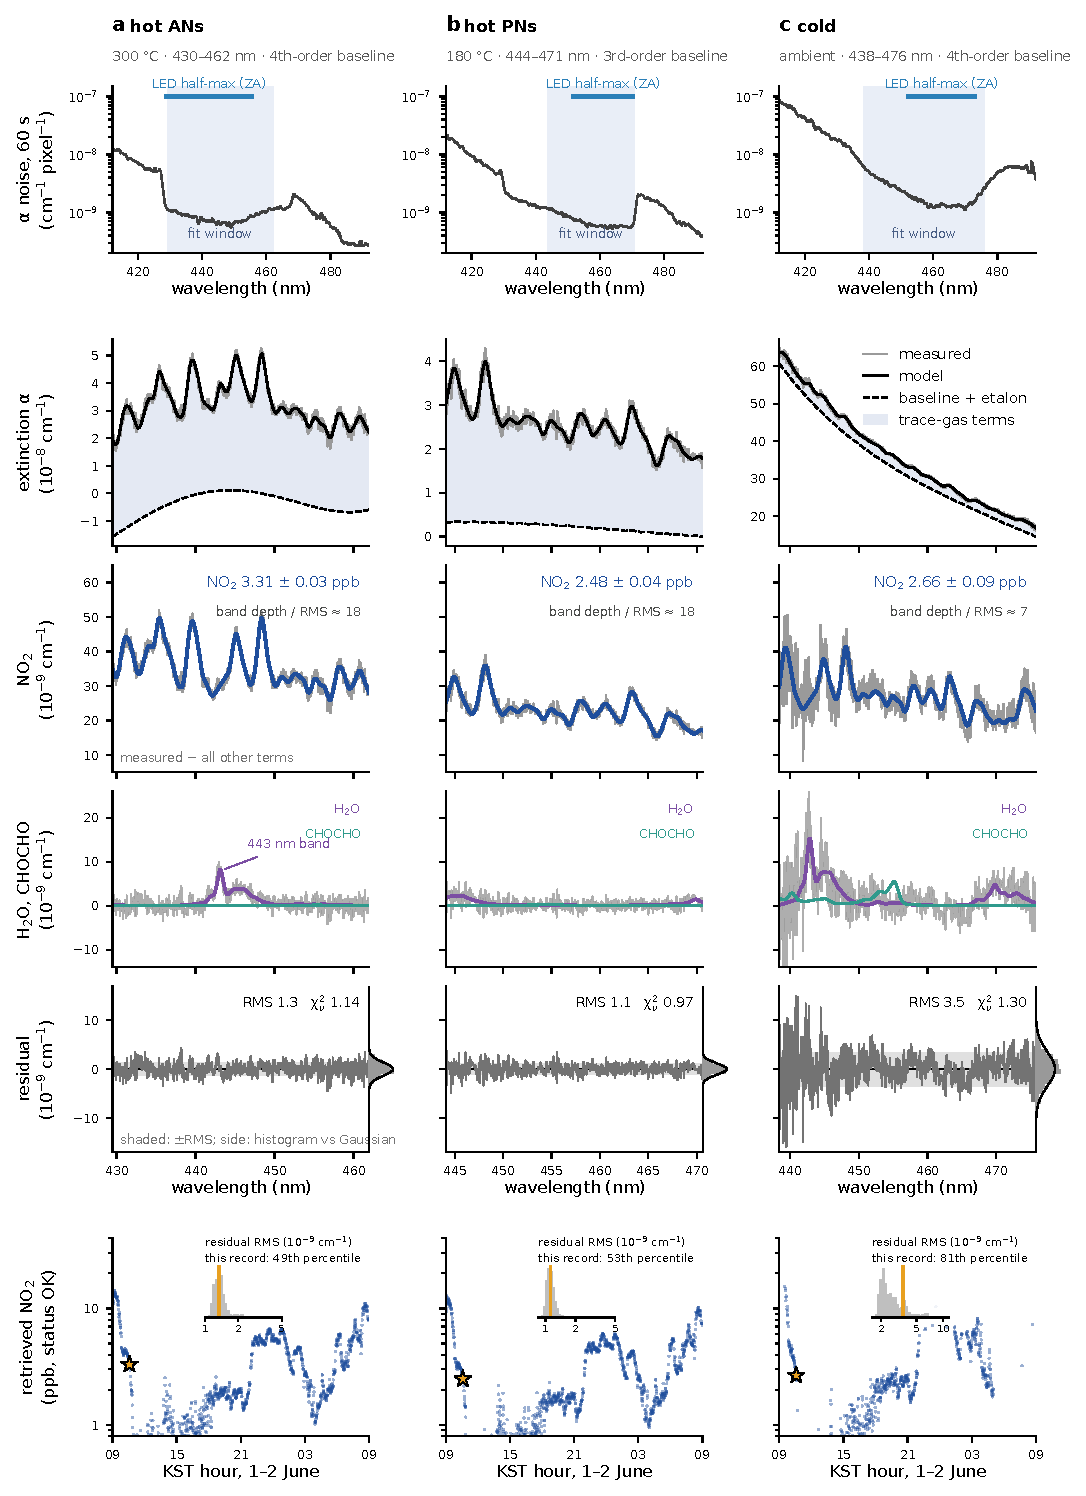
\includegraphics[width=\textwidth,height=0.66\textheight,keepaspectratio]{figures/fig02.pdf}
\caption{One record (1 June 2026, 10:35 KST; cold channel 10:34:34) retrieved in the three
configurations of Table~\ref{tab:1}. Columns: \textbf{(a)} hot ANs (300\,$^{\circ}$C), \textbf{(b)} hot PNs (180\,$^{\circ}$C), \textbf{(c)} cold.
\textbf{Top row:} per-pixel noise of the 60\,s extinction spectrum in the hour around the record, with the fit window
shaded. Each window sits on the low-noise band set by its LED (bar: LED emission half-maximum from zero-air
spectra); the cold window extends 13\,nm below its LED half-maximum, where the noise is several times higher; the step at 428\,nm in (a) is the band-pass filter edge and the step at 470\,nm in (b) is the
red edge of the 469\,nm LED. \textbf{Middle block,} top to bottom: measured extinction with the fitted model and the
baseline-plus-etalon term (shading: sum of trace-gas terms); the NO$_2$ contribution, shown as the measurement minus
every other fitted term, with the fitted NO$_2$ term; the same for H$_2$O, with the fitted CHOCHO term; and the
residual, with $\pm$RMS shaded and its histogram against a Gaussian of the same RMS at right. The lower three rows share
one vertical scale across columns. Values in the NO$_2$ row are the operational retrieval and its reported 1$\sigma$;
``band depth / RMS'' is the peak-to-peak of the fitted NO$_2$ term divided by the residual RMS. \textbf{Bottom row:}
the NO$_2$ retrieved by the same configuration over the surrounding 24\,h (fits with reduced $\chi^2 \le 1.5$; $n = \fieldnum{1397}$, \fieldnum{1399}, \fieldnum{707}),
the star marking this record; inset: distribution of residual RMS over those fits, on which this record sits at the
\fieldnum{49}th, \fieldnum{53}rd and \fieldnum{81}st percentile.}
\label{fig:2}
\end{figure*}

\subsection{Recovery of a known truth}
\label{sec:3.1}

Spectra are generated from the forward model of Sect.~\ref{sec:2.1} with prescribed gas
amounts, a Chebyshev baseline, a wavelength shift and a squeeze, and retrieved
with the same model. Over 27 combinations -- nine shifts from $-4$ to $+4$\,px (including sub-pixel
values of $\pm0.37$\,px) crossed with squeezes of 0.998, 1.000 and 1.002 -- the largest error in the retrieved NO$_2$ amount is
$9.5\times10^{-13}$ relative and the largest error in the recovered shift $6.7\times10^{-10}$\,px. The
retrieval reproduces its own forward model to machine precision, which is a
statement about the solver and not about the instrument.

The baseline order is the one structural choice the retrieval makes on its
own. Sweeping it from 0 to 8 on a noise-free spectrum built with a
fourth-order baseline, the retrieved NO$_2$ is in error by 27\,\% at order 0 and
0.75\,\% at order 1, and reaches machine precision at order 2 and above; the
normalised condition number rises from 14.9 to 33.8 across the sweep and the
degrees of freedom fall from 543 to 535. On noisy realisations of the same
spectrum the scatter of the retrieved NO$_2$ is 0.88 to 0.91 times the reported
1$\sigma$ at order 2 and above. For this configuration, with white photon noise and a correct model, the
reported uncertainty is accurate to about ten per cent -- which is the
baseline against which the structural terms of Sect.~\ref{sec:4} should be read (Fig.~\ref{fig:3}a, b). It is a
statement about one configuration: across the 13 synthetic instruments of Fig.~\ref{fig:1}a the white-noise ratio
ranges from 0.91 to 1.32, and at nominal noise it lies between 1.22 and 1.32 in 9 of them, where the free
wavelength shift adds scatter the covariance does not carry (Sect.~\ref{sec:3.4}).

\begin{figure*}[t]
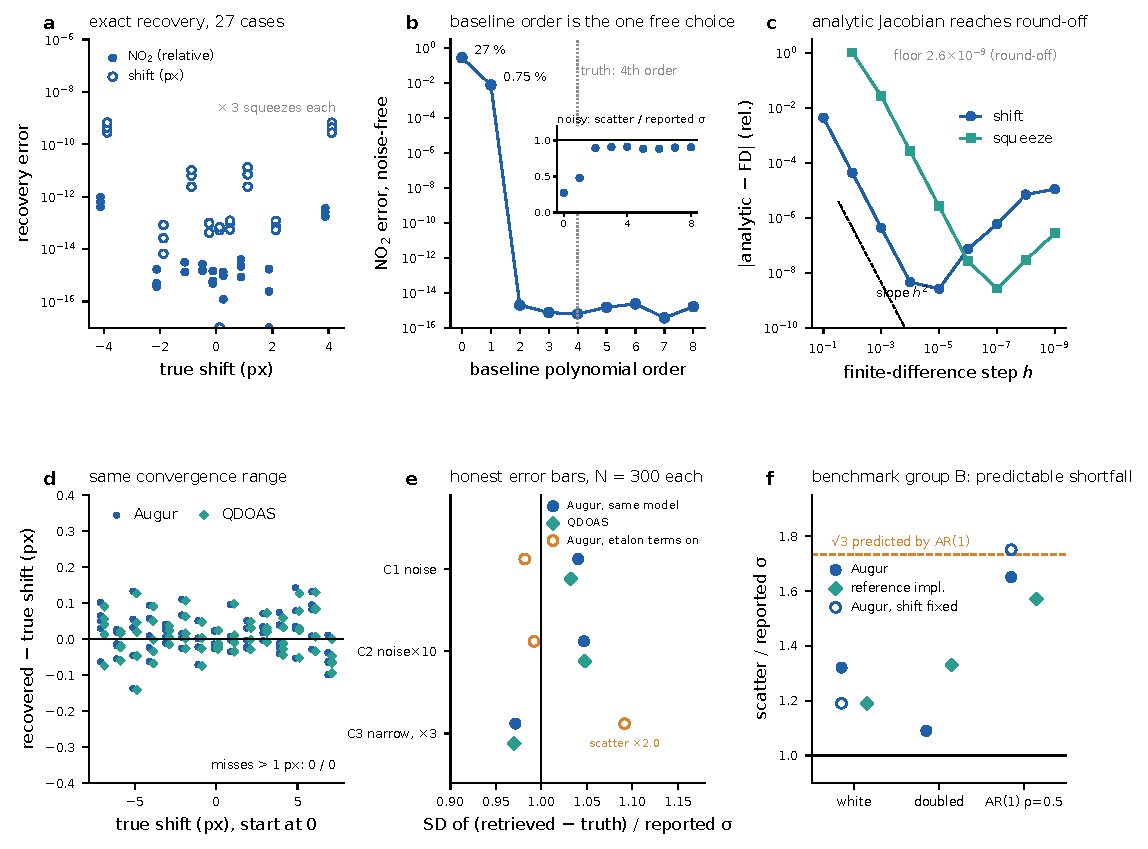
\includegraphics[width=\textwidth]{figures/fig03.pdf}
\caption{Validation of the retrieval core. \textbf{(a)} Error in the recovered NO$_2$ amount (filled, relative) and
wavelength shift (open, px) for 27 noise-free spectra: nine shifts between $-4$ and $+4$\,px, each with squeezes 0.998, 1.000
and 1.002. \textbf{(b)} Error in NO$_2$ against the order of the fitted baseline for a noise-free spectrum built with a
fourth-order baseline; inset, on noisy realisations of the same spectrum, the realised scatter of NO$_2$ divided by the
reported 1$\sigma$. \textbf{(c)} Difference between the analytic Golub--Pereyra Jacobian and a central finite difference of the
projected residual, against the finite-difference step, for the shift and the squeeze; the dashed line has slope $h^2$.
\textbf{(d)} Shift recovered by Augur and by QDOAS minus the true shift, for true shifts from $-7$ to $+7$\,px (five noisy
realisations each, both started at 0). \textbf{(e)} Standard deviation of (retrieved $-$ true)/reported $\sigma$ over 300 realisations
in each of three conditions (measurement noise; ten times that; a narrow window with three times the noise), for Augur
and QDOAS fitting the same model, and for Augur with its etalon terms switched on. \textbf{(f)} Benchmark group B: realised
scatter divided by the reported uncertainty under white, doubled and autocorrelated (AR(1), $\rho = 0.5$) noise, for Augur,
for the benchmark's reference implementation and for Augur with the shift fixed at its true value; the dashed line is the
$\sqrt{3}$ inflation predicted for $\rho = 0.5$.}
\label{fig:3}
\end{figure*}

\subsection{The analytic Jacobian}
\label{sec:3.2}

The two-term Golub--Pereyra derivative of Sect.~\ref{sec:2.3} is compared against a central
finite difference of the projected residual, evaluated inside a real fit
rather than on a constructed test function: the optimiser call is intercepted
and the analytic Jacobian it was handed is differenced against the residual it
was minimising. An invariant check of this form runs on every fit in the test
suite at the solver's default step; what is reported here is the step-size
sweep (Table~\ref{tab:jacobian_steps}), which is what turns a passing check into a measurement.

\begin{table}[t]
\caption{Difference between the analytic Golub--Pereyra Jacobian and a central finite difference of the projected residual, evaluated inside a real fit, against the finite-difference step $h$, for the shift (px) and the squeeze. Bold: the minimum of each column.}
\label{tab:jacobian_steps}
\begin{tabular}{lll}
\tophline
step $h$ & shift (px) & squeeze \\
\middlehline
$10^{-1}$ & $4.31\times10^{-3}$ & outside the box \\
$10^{-2}$ & $4.29\times10^{-5}$ & 1.02 \\
$10^{-3}$ & $4.29\times10^{-7}$ & $2.63\times10^{-2}$ \\
$10^{-4}$ & $4.51\times10^{-9}$ & $2.61\times10^{-4}$ \\
$10^{-5}$ & $\mathbf{2.60\times10^{-9}}$ & $2.61\times10^{-6}$ \\
$10^{-6}$ & $7.28\times10^{-8}$ & $2.61\times10^{-8}$ \\
$10^{-7}$ & $5.79\times10^{-7}$ & $\mathbf{2.64\times10^{-9}}$ \\
$10^{-8}$ & $6.95\times10^{-6}$ & $2.87\times10^{-8}$ \\
$10^{-9}$ & $1.09\times10^{-5}$ & $2.70\times10^{-7}$ \\
\bottomhline
\end{tabular}
\end{table}

Both parameters give the expected V (Fig.~\ref{fig:3}c). The truncation branch falls with a fitted
slope of $+2.001$ in each, which is the $h^2$ of a central difference, and the
round-off branch rises again as the difference of two nearly equal numbers
loses significance. The minima are $2.60\times10^{-9}$ for the shift and
$2.64\times10^{-9}$ for the squeeze, a ratio of 1.018: the two parameters reach
the same floor, which is the signature of a floor set by round-off in the
shared residual evaluation rather than by any error in either derivative.

This is a stronger statement than agreement at one step size. An analytic
expression that omitted a term -- the one-term approximation of \citet{Kaufman_1975}, which drops the derivative of the projector, is the natural candidate
-- would agree with the finite difference only down to the size of the omitted
term and would then flatten, not descend to the round-off floor. The descent
is what identifies the expression being differentiated as the derivative
itself.

The two parameters must be swept separately. The shift is measured in pixels
and is $O(1)$, while the squeeze is a multiplier near unity constrained to a
box of order $\pm 0.02$, so $h = 10^{-2}$ is already half the box for the
squeeze and the entry there is a bound artefact rather than a failure of the
derivative. A combined maximum over both parameters would show 1.02 at that
step and hide the V.

\subsection{An independent implementation of the same problem}
\label{sec:3.3}

QDOAS \citep{Danckaert_2017} solves the same separable least-squares problem by a
different route: Marquardt--Levenberg with a singular-value decomposition and a
numerically differenced Jacobian, against Augur's variable projection with an
analytic projected Jacobian. It does not know about cavities, so the
comparison is made by presenting the extinction spectrum as a virtual
transmission, $I = \exp(-K\alpha)$ with $I_0 = 1$, whereby the optical depth QDOAS
forms is exactly $K\alpha$ and the two codes are solving the same equations on
the same numbers.

On noise-free synthetic spectra with shifts of 0, $-1.96$, $+2$ and $-4$\,px, Augur
recovers NO$_2$ to $9.5\times10^{-13}$ relative and QDOAS to $5.0\times10^{-3}$, the latter limited by
its output resolution rather than by its algorithm; QDOAS recovers the shift
to within 0.0042\,px. On 30 noisy realisations the two codes have
root-mean-square relative errors of 0.0042 and 0.0045 against the same truth,
and differ from each other by at most $5.7\times10^{-3}$ relative in NO$_2$. On the field record (53 days), with each spectrum's measured temperature and pressure used
for the unit conversion and records selected by an NO$_2$-conditional $\chi^2$ envelope, the NO$_2$ amounts of the
two codes agree with $r^2 \ge \fieldnum{0.990}$ in all three configurations (Table~\ref{tab:qdoas_field}). The agreement is
not a scale identity: the Deming slope QDOAS/Augur is \fieldnum{1.039} in the cold configuration and \fieldnum{1.063} and
\fieldnum{1.043} in the 180 and 300\,$^{\circ}$C configurations, where $r^2 = \fieldnum{1.000}$, so the two codes differ in the
heated-channel NO$_2$ scale by \fieldnum{4}--\fieldnum{6}\,\% for a reason we have not identified. The weak absorbers agree less
well (CHOCHO $r^2$ \fieldnum{0.889}--\fieldnum{0.959}, slope \fieldnum{0.81}--\fieldnum{1.19}; H$_2$O slope \fieldnum{1.04}--\fieldnum{1.38}).

\begin{table}[t]
\caption{Agreement of QDOAS with Augur on the field record, per retrieval configuration and species: number of
records $n$ in the NO$_2$-conditional $\chi^2$ envelope, Deming slope QDOAS/Augur ($\lambda = 1$) and $r^2$. The
unit conversion uses each spectrum's measured temperature and pressure.}
\label{tab:qdoas_field}
\begin{tabular}{lllll}
\tophline
configuration & species & $n$ & Deming slope & $r^2$ \\
\middlehline
cold & NO$_2$ & \fieldnum{36\,241} & \fieldnum{1.039} & \fieldnum{0.990} \\
cold & CHOCHO & \fieldnum{36\,241} & \fieldnum{0.807} & \fieldnum{0.889} \\
cold & H$_2$O & \fieldnum{36\,241} & \fieldnum{1.377} & \fieldnum{0.887} \\
hot PNs (180\,$^{\circ}$C) & NO$_2$ & \fieldnum{73\,916} & \fieldnum{1.063} & \fieldnum{1.000} \\
hot PNs (180\,$^{\circ}$C) & CHOCHO & \fieldnum{73\,916} & \fieldnum{1.195} & \fieldnum{0.914} \\
hot PNs (180\,$^{\circ}$C) & H$_2$O & \fieldnum{73\,916} & \fieldnum{1.042} & \fieldnum{0.974} \\
hot ANs (300\,$^{\circ}$C) & NO$_2$ & \fieldnum{74\,539} & \fieldnum{1.043} & \fieldnum{1.000} \\
hot ANs (300\,$^{\circ}$C) & CHOCHO & \fieldnum{74\,539} & \fieldnum{1.054} & \fieldnum{0.959} \\
hot ANs (300\,$^{\circ}$C) & H$_2$O & \fieldnum{74\,539} & \fieldnum{1.038} & \fieldnum{0.981} \\
\bottomhline
\end{tabular}
\end{table}

In a
larger test with 300 realisations in each of three noise conditions, the
standard deviation of the error normalised by the reported uncertainty is 0.97
to 1.05 for both codes when they fit the same model, and started from zero both
recover true shifts between $-7$ and $+7$\,px with no miss larger than a pixel
(Fig.~\ref{fig:3}d, e). Switching on Augur's etalon terms in the narrow window doubles the
scatter there -- a choice of model, not a property of the solver.

The conclusion drawn from this in Sect.~\ref{sec:2.9} is therefore narrower than identity: on
synthetic spectra the two codes return the same concentrations, and on field spectra they agree in NO$_2$
to within a scale difference of a few per cent. Where they diverge most -- the wavelength shift in the cold
window, and with it the weak absorbers there (Sect.~\ref{sec:5.1}) -- the data do not determine the shift, so
neither code's value is established by its fit.

\subsection{A benchmark that others can run}
\label{sec:3.4}

The comparison of Sect.~\ref{sec:3.3} is specific to one pair of codes and one set of cross
sections. To make the same measurements repeatable elsewhere we release a
synthetic benchmark of 261 cases in six groups: exact recovery with no noise
(A), reported uncertainty against realised scatter under white, doubled and
autocorrelated noise (B), bias from a deliberately incomplete model (C), cases
whose wavelength shift is not determined by the data (D), the same truth
presented in two fitting windows (E), and the cost of the sub-pixel
interpolator against band-limited truth (F). Truth is known by construction,
the spectra are built from the instrument's own cross sections and wavelength
calibration but contain no retrieval code, and the generator is deterministic
under a stated seed.

Group B is worth reporting in full, because its result is not the one the
paper's own closure test gives and the difference is instructive. Augur
returns scatter-to-reported ratios of 1.32, 1.09 and 1.65 for white, doubled
and autocorrelated noise, against 1.19, 1.33 and 1.57 from the reference
implementation: both codes pass one condition of three, and they fail
different ones. Two effects account for the pattern. Fixing the wavelength
shift at its true value brings Augur's white-noise ratio from 1.32 to 1.19,
which is the reference implementation's value, so the difference between the
two codes under white noise is the nonlinear degree of freedom and the size of
the box it is searched in, not the covariance they propagate. And the
correlated-noise result is predicted by the noise model rather than being a
property of either code: an AR(1) residual with $\rho = 0.5$ inflates the
variance of a sum by $(1+\rho)/(1-\rho) = 3$, so a covariance built on an
independence assumption must understate the scatter by $\sqrt{3} = 1.73$. The
measured 1.57 and 1.65 sit just below it, and fixing the shift moves Augur to
1.75 -- the free shift had been absorbing part of the correlated structure
(Fig.~\ref{fig:3}f).

This is the benchmark doing what it was built for. The shortfall under
correlated noise is not a defect to be repaired in either implementation; it
is the reported uncertainty answering a question about photon statistics when
the residual is not photon statistics, and its size is calculable in advance.

A reference implementation is included, and its scorecard is the example
against which a submission is read. It is a deliberately plain profiled grid
search, not a production retrieval, and the benchmark is not a ranking: groups
C and E are reported rather than passed or failed, because the quantity they
measure is not one any implementation is expected to cover.

\subsection{Relative scale between the two hot channels}
\label{sec:3.5}

The alkyl nitrate product is a difference between two channels, so their
relative scale enters it directly. NO$_2$ was injected into both heated channels, with both ovens at their
operating temperatures, at two concentration steps on 2026-08-10/11. The steps did not equilibrate (the
delivery line was still passivating), so only the ratio between the channels is used. In the original
processing the median of the per-record ratios was 1.2278 at the lower step and 1.2276 at the higher (the
median channel readings were 14.75 and 11.97\,ppb, and 71.57 and 58.16\,ppb; ratios of these medians are 1.2322
and 1.2306), and an origin regression over the 58 one-minute means of one file gives a slope of 0.81666
with $r^2$ 0.9998. Reprocessed with the current code, block 2053 reads 1.239 times block 4101
(interquartile range 1.231--1.255, $n = 41$ records with block 4101 above 20\,ppb).

This establishes that the relative scale is constant over the range tested. It does not give the scale
used in the campaign product: the laboratory ratio describes the calibration state of August, and the
product uses $g' = \fieldnum{0.952}$ for 18 May--5 June, from a field injection. Nor does it establish the absolute
recovery of either channel, or separate optical from thermal causes of the offset between the channels,
because both cells were at their operating temperatures throughout.

\subsection{What is not verified here}
\label{sec:3.6}

A comparison with a co-located reference analyser exists, and it bounds what this paper can claim.
Against the NIER air-quality-monitoring NO$_2$ analyser at the site (molybdenum-converter type), the
operational NO$_2$ of the heated channels has ordinary-least-squares gains of \fieldnum{0.57} (180\,$^{\circ}$C) and \fieldnum{0.65}
(300\,$^{\circ}$C), while the ambient-temperature channel has \fieldnum{0.92}--\fieldnum{1.00}; the median ratio of heated to
ambient-temperature NO$_2$ is \fieldnum{0.72}, although the heated channels measure NO$_2$ plus thermally produced NO$_2$
and should read at least as high. A laboratory injection with the ovens at 300 and 180\,$^{\circ}$C gave a block-2053
sensitivity of at least 1.08 relative to the cylinder, so oven temperature alone does not explain the
discrepancy, and its cause is unresolved. It is a multiplicative error that leaves the residual, the reported
uncertainty and every context field proposed in Sect.~\ref{sec:6} unchanged -- an instance of the class of error
this paper is about, not a property of the spectral fit. No absolute accuracy is claimed. The verification of Sects.~\ref{sec:3.1}
and \ref{sec:3.3} is of the retrieval against its own forward model and against another
implementation of that model, which bounds implementation error but not model
error -- and model error is precisely what Sect.~\ref{sec:3.4} measures on the benchmark.

%% Sect. 4 -- from augur_AMT_§4 draft v16 (2026-09-22); condensed 2026-09-29 (denominator discussion -> Appendix D;
%% Sect. 4.6 replaced by the discussion of previous uncertainty treatments; the three-number prescription is in Sect. 6.1).
\section{Structural error budget}
\label{sec:4}

\subsection{What the fit reports, and what it cannot report}
\label{sec:4.1}

The covariance returned by the fit (Sect.~\ref{sec:2.5}) propagates only the residual scatter of the spectrum being
fitted. For the operational configuration it gives a single-scan reported uncertainty of \fieldnum{0.55}\,\% on the channel
NO$_2$ amount, the number that appears in the data product. Three inputs of Eq.~(\ref{eq:1}) are not measured with
the spectrum but interpolated to its time from neighbouring calibration blocks: the zero-air reference $I_0$, the
mirror reflectivity $R(\lambda,t)$, and the etalon frequency $f$, which is held fixed rather than redetermined per
scan. An error in any of these enters $\alpha$ directly and, within a single fit, is indistinguishable from a change
in the gas amounts; the residual does not see it, so the reported uncertainty does not contain it.

Of two further inputs, sample temperature and pressure contribute negligibly and the instrument line shape could not
be tested adequately. Temperature and pressure, interpolated the same way as $I_0$, contribute below \fieldnum{0.1}\,\%. The kernel is resampled onto the
detector grid with a radius of $\lfloor 4\sigma \rfloor + 1$ pixels, and at the mismatch measured in the
ambient-temperature channel (FWHM 0.765 against 0.785\,nm) the retrieved amount moved by $\sim 10^{-5}$\,\%. This shows only
that the test did not carry a width change of that size into the forward model; a test with a continuously resampled kernel has not been made, and no mismatch was measured for
the heated channels. The residual does carry a signal-proportional model error: the median reduced $\chi^2$ of the
300\,$^{\circ}$C channel rises from \fieldnum{1.05} at NO$_2$(180\,$^{\circ}$C) below 1\,ppb to \fieldnum{1.57} at 10--20\,ppb. That error
is not in the budget below; the cross sections and the line shape are candidates.

\subsection{Measuring a structural term}
\label{sec:4.2}

A structural term is measured by perturbing an input the way the operational pipeline can actually be wrong,
re-running the full retrieval and reading the change in the retrieved amount. In leave-one-out (LOO) perturbation,
a jackknife-type resampling of the calibration record \citep{Efron_1979}, one calibration knot is removed, the remaining
knots are re-interpolated across the gap, and every scan in it is re-retrieved. Because the interpolated interval is
roughly doubled relative to operation, LOO is an upper bound by construction for the interpolation terms (scope in
Sect.~\ref{sec:4.4}). In the split-half estimate, each calibration block
is split into contiguous (first and second half) or interleaved (even and odd scans) halves, and the difference of
the two block means measures the knot noise with no change of interval. With $n/2$ scans per half the difference
carries a factor of two relative to the full-block knot noise, which is divided out.

The ratio of the two estimates separates knot noise from curvature (Table~\ref{tab:splithalf_loo}). A ratio near unity
means the LOO error is entirely knot noise and a shorter reference interval would not improve it; a ratio near one
half means the interval carries curvature. For the 180\,$^{\circ}$C channel the ratio is \fieldnum{0.74}--\fieldnum{0.91}, so
measuring the references more often, as recommended qualitatively by \citet{Washenfelder_2008}, would reduce the
error little, and averaging more scans per block is the lever that could. For the 300\,$^{\circ}$C channel
(\fieldnum{0.40}--\fieldnum{0.43}) the interval carries curvature, and shorter intervals would help. The ordering agrees with the
direct measurement of Sect.~\ref{sec:6.2}: tripling the reflectivity interval from 2 to 6\,h raises the interpolation
error by \fieldnum{15}\,\% in hot PNs and by \fieldnum{33}\,\% in hot ANs. Contiguous and interleaved halves give similar knot noise
in the NO$_2$ amount (the contiguous estimate is \fieldnum{7}--\fieldnum{19}\,\% smaller), so the interleaved split does not
understate it.

\begin{table}[t]
\caption{Zero-air reference-interpolation error in the channel NO$_2$ amount (per cent) from the split-half estimate
of knot noise, with contiguous and interleaved halves, and from leave-one-out (LOO) knot removal, and the ratio
split-half/LOO. Hot channels: the 157 zero-air knots of 18--24 May, current fit settings and clock-aligned
reflectivity.}
\label{tab:splithalf_loo}
\begin{tabular}{lllll}
\tophline
channel & split-half, contiguous & split-half, interleaved & LOO & ratio \\
\middlehline
hot PNs & \fieldnum{1.437}\,\% & \fieldnum{1.782}\,\% & \fieldnum{1.95}\,\% & \fieldnum{0.74}--\fieldnum{0.91} \\
hot ANs & \fieldnum{0.90}\,\% & \fieldnum{0.97}\,\% & \fieldnum{2.25}\,\% & \fieldnum{0.40}--\fieldnum{0.43} \\
\bottomhline
\end{tabular}
\end{table}

\subsection{Terms must be propagated jointly, and the scale taken once}
\label{sec:4.3}

Measuring each term separately and adding the results in quadrature fails here for two different reasons. First,
model-space and $\alpha$-space perturbations are not additive. Perturbing $I_0$ and perturbing $R$ both move $\alpha$,
and their effects add scan by scan: the median of $|\,\delta_{\mathrm{joint}} - (\delta_{I_0} + \delta_{R})\,|$ is
\fieldnum{0.8}--\fieldnum{2.2}\,\% of the signal. The etalon's sine and cosine columns, in contrast, are free linear parameters
that absorb part of any smooth perturbation of $\alpha$ before it reaches the gas columns. Perturbing all three
simultaneously therefore gives a smaller result than summing the three responses, by \fieldnum{8.3}\,\% (hot ANs),
\fieldnum{6.4}\,\% (hot PNs) and \fieldnum{$-0.2$}\,\% (cold). Adding the etalon term as if it were independent overestimates by an
amount that depends on the fitting window and polynomial order.

Second, the joint scale differs from any quadrature combination of the single-term scales, whether robust scales or
standard deviations are combined. Combining median-based scales in quadrature misses the directly
measured joint scale by \fieldnum{$+13.3$}\,\% (hot ANs), \fieldnum{$-8.1$}\,\% (hot PNs) and \fieldnum{$+6.9$}\,\% ($\Sigma$ANs). The same
combination on standard deviations does not repair it: the joint exceeds the quadrature sum by \fieldnum{15.5}\,\% for the
ANs channel and \fieldnum{7.6}\,\% for $\Sigma$ANs, and falls \fieldnum{2.5}\,\% below it for PNs. For variances the failure has two
measured parts. The single-term responses of $\Sigma$ANs are correlated (pairwise $r = \fieldnum{0.25}$, \fieldnum{0.18} and
\fieldnum{0.03}), which adds \fieldnum{28.7}\,\% to the sum of their variances, and the terms do not superpose (the etalon
interaction above), which removes \fieldnum{12.9}\,\%, leaving the joint variance \fieldnum{15.8}\,\% above the sum. Robust scales
fail in addition through distribution shape. The normalised shape statistic $s = 1.4826\,\mathrm{MAD}/\mathrm{SD}$ is unity for a Gaussian and 0.727 for a Laplace.
The three $\Sigma$ANs components have $s = \fieldnum{0.73}$ ($I_0$), \fieldnum{0.32} ($R$) and \fieldnum{0.98} (etalon), and the joint series
has a fourth shape again ($s = \fieldnum{0.56}$), so a median-based scale captures a different fraction of the variance in each.

Because the sign and size of the discrepancy depend on covariance, interaction and shape that are known only after
the joint propagation, no correction factor can replace it. The rule used throughout this paper is therefore to
propagate every term simultaneously into the final product time series, and to take the scale once, at the end,
with the same estimator used for the quantity it will be compared against.

\subsection{The budget}
\label{sec:4.4}

Table~\ref{tab:2} gives the budget as the robust scale and standard deviation of the jointly propagated response, in
mixing-ratio units. The $\Sigma$ANs row is propagated through the channel
difference rather than formed from the channel rows (Sect.~\ref{sec:4.3}). The record evaluated is the product
reprocessed on the clock-aligned reflectivity reference (Sect.~\ref{sec:5.4}), not the dataset delivered to the
campaign, which was produced before that correction and is retained as delivered. Records whose perturbed fit
terminated at a parameter bound are excluded, because such a fit has not converged (Sect.~\ref{sec:5.2}). The cold
channel was not re-run on this basis and is not included.

\begin{table*}[t]
\caption{Structural error budget, ppb, from a single propagation over the 60\,s ambient records of
2026-05-18..05-24 on the clock-aligned reflectivity reference (Sect.~\ref{sec:5.4}): of the \fieldnum{9034} records with a
reflectivity knot within 1\,h, the \fieldnum{187} in which a fit of either channel terminated at a bound are excluded
(Sect.~\ref{sec:5.2}), leaving \fieldnum{8847}. $\Sigma$ANs is formed as in the product, 300\,$^{\circ}$C minus $g'$ times
180\,$^{\circ}$C with $g' = \fieldnum{0.9524}$ for this period. Columns $I_0$, $R$, $f$: single-term responses; joint: simultaneous response, the quantity to be used. rSD: robust scale
($1.4826\,$MAD); SD: standard deviation; $s$: shape statistic of Sect.~\ref{sec:4.3}.}
\label{tab:2}
\begin{tabular}{llllll}
\tophline
 & & $I_0$ & $R$ & $f$ & joint \\
\middlehline
hot ANs channel & rSD & \fieldnum{0.0437} & \fieldnum{0.0350} & \fieldnum{0.0082} & \fieldnum{0.0641} \\
 & SD & \fieldnum{0.0600} & \fieldnum{0.0829} & \fieldnum{0.0086} & \fieldnum{0.1186} \\
 & $s$ & \fieldnum{0.73} & \fieldnum{0.42} & \fieldnum{0.95} & \fieldnum{0.54} \\
hot PNs channel & rSD & \fieldnum{0.0416} & \fieldnum{0.0126} & \fieldnum{0.0187} & \fieldnum{0.0435} \\
 & SD & \fieldnum{0.0428} & \fieldnum{0.0384} & \fieldnum{0.0189} & \fieldnum{0.0590} \\
 & $s$ & \fieldnum{0.97} & \fieldnum{0.33} & \fieldnum{0.99} & \fieldnum{0.74} \\
$\Sigma$ANs & rSD & \fieldnum{0.0558} & \fieldnum{0.0269} & \fieldnum{0.0191} & \fieldnum{0.0693} \\
 & SD & \fieldnum{0.0768} & \fieldnum{0.0831} & \fieldnum{0.0195} & \fieldnum{0.1236} \\
 & $s$ & \fieldnum{0.73} & \fieldnum{0.32} & \fieldnum{0.98} & \fieldnum{0.56} \\
\bottomhline
\end{tabular}
\end{table*}

The reflectivity term dominates the tail of the budget and the zero-air term its typical record. Of the single-term quadrature sum for $\Sigma$ANs, $I_0$ carries \fieldnum{74}\,\% on
the robust scale but \fieldnum{45}\,\% in standard deviation, while $R$ carries \fieldnum{17}\,\% and \fieldnum{52}\,\%. The reflectivity term
is small for a typical record and the largest contributor overall, because its error is concentrated in a few
intervals: five of the \fieldnum{155} hours in the window carry \fieldnum{57}\,\% of its variance (Fig.~\ref{fig:4}a, c).
Section~\ref{sec:6} uses this contrast to choose between remedies.

\begin{figure*}[t]
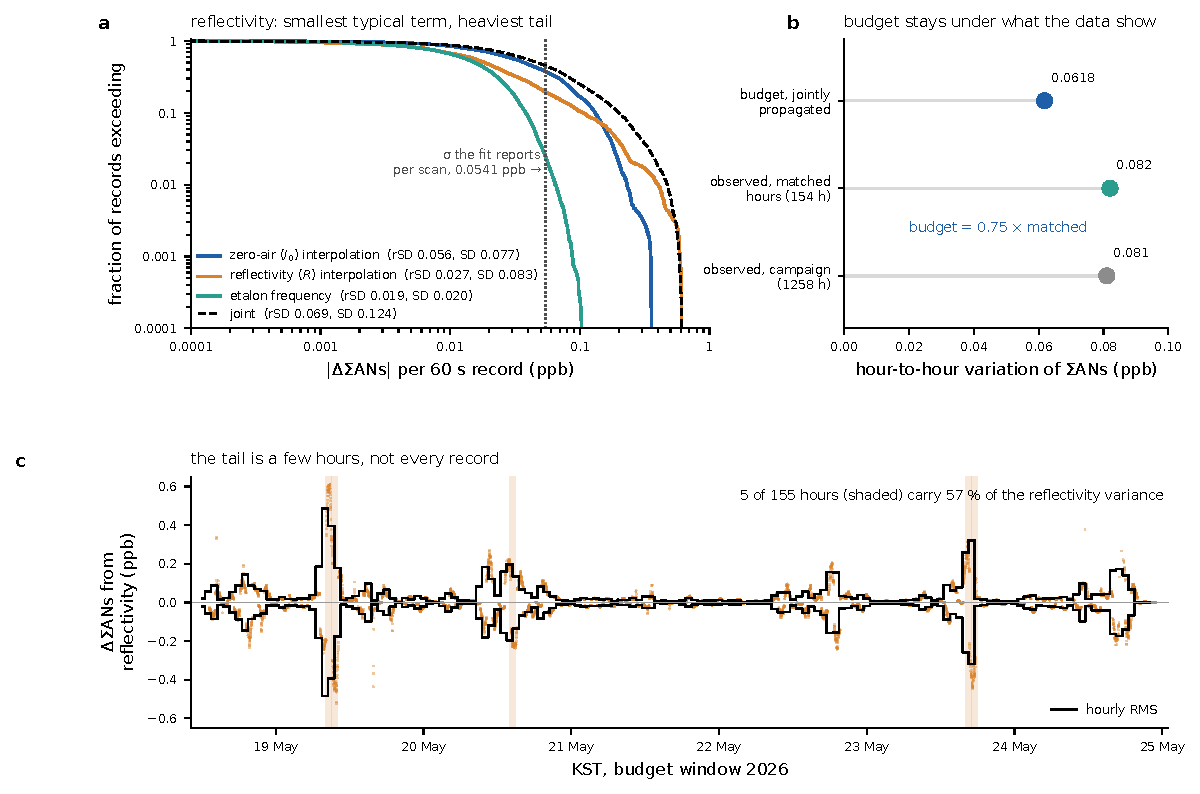
\includegraphics[width=\textwidth]{figures/fig04.pdf}
\caption{Structural error budget of the alkyl nitrate product over the \fieldnum{8847} records of 18--24 May ($g' =
\fieldnum{0.9524}$). \textbf{(a)} Fraction of records whose $\Sigma$ANs changes by more than a given amount for each reference term
alone and all three jointly; legend: robust scale and standard deviation (Table~\ref{tab:2}); dotted: the per-scan fit
uncertainty. \textbf{(b)} Hour-to-hour variation predicted by the joint budget and observed in the matched hours and over
the campaign. \textbf{(c)} Reflectivity term per record (points) and hourly RMS (steps); shaded, the five hours that carry
\fieldnum{57}\,\% of its variance.}
\label{fig:4}
\end{figure*}

The budget describes the instrument when its calibration is working. A perturbation experiment can only be run on
scans that have neighbouring knots of both reference types, so periods in which the calibration itself failed, which
are the periods with the largest errors, are absent from it. The budget window is the best-covered stretch of the
deployment, with no record outside the knot range and no gap longer than two hours; over the campaign \fieldnum{11.03}\,\% of
cold records lie in such gaps (Sect.~\ref{sec:5.3}).

Against what the fit reports, the budget is large. A budget record is one 60\,s ambient bin, which at the
operational scan rate is one scan, and the median fit-propagated $\Sigma$ANs uncertainty at that resolution, over the
same records, is \fieldnum{0.0541}\,ppb. The structural contribution alone is therefore \fieldnum{1.28} times the reported sigma on the
robust scale and \fieldnum{2.29} times it in standard deviation. The total uncertainty is \fieldnum{1.63} to \fieldnum{2.50} times what the
fit reports, the range spanning the two scales rather than any doubt about the measurement. Because
leave-one-out doubles the interpolation interval (Sect.~\ref{sec:4.2}), these are upper-bound estimates for the
interpolation terms in the best-calibrated week of the deployment. They exclude terms common to all knots (cross
sections, Rayleigh scattering, the reflectivity scale) and periods of failed calibration, and are not a campaign-wide bound. The per-scan fit uncertainty is the
appropriate denominator; the uncertainty column shipped with the product, the five-minute fit uncertainty and the
zero-air scatter answer different questions (Appendix~\ref{app:D}, Table~\ref{tab:denominators}).

\subsection{Consistency with the observed variation}
\label{sec:4.5}

The budget can be checked against the data it claims to describe. A channel-differential term must appear in the
channel-difference product, and a term that varies on the timescale of the calibration interval must appear in the
hour-to-hour variation of that product. The observed variation is an upper bound on the measurement error, because
it also contains atmospheric variability. Both sides pass through the same estimator,
$1.4826\,\mathrm{median}|\Delta|/\sqrt{2}$ over adjacent hourly means, and the budget series is itself hourly (median
spacing \fieldnum{1.00}\,h, $p_{90}$ \fieldnum{1.03}\,h), so the comparison is made on the same timestamps, paired
(Table~\ref{tab:hourly_check}). The lag-1 autocorrelation is \fieldnum{$-0.60$} for the budget, because removing a knot pins the interpolant at the two
neighbours and forces it to depart on alternate sides, and \fieldnum{$+0.73$} for the observation in the matched hours, from
atmospheric persistence.

\begin{table}[t]
\caption{Hour-to-hour variation of hourly $\Sigma$ANs, summarised by $1.4826\,\mathrm{median}|\Delta|/\sqrt{2}$ (ppb), observed and predicted by the budget, and the ratio of the budget to the observed statistic in the matched hours.
Observed: the clock-aligned $\Sigma$ANs product (quality flag below 2), hourly means of at least 8 records.}
\label{tab:hourly_check}
\begin{tabular}{lll}
\tophline
 & gate statistic (ppb) & ratio \\
\middlehline
observed, campaign (\fieldnum{1258}\,h) & \fieldnum{0.081} & -- \\
observed, hours matched to the budget (\fieldnum{154}\,h) & \fieldnum{0.082} & -- \\
budget, hourly, jointly propagated, matched hours & \fieldnum{0.0618} & \fieldnum{0.75} \\
budget, at record resolution & \fieldnum{0.0693} & \fieldnum{0.84} \\
\bottomhline
\end{tabular}
\end{table}

The budget predicts \fieldnum{0.75} times the observed hour-to-hour variation (Fig.~\ref{fig:4}b), evaluated on the same
\fieldnum{154} matched hours and \fieldnum{153} consecutive pairs against \fieldnum{0.082}\,ppb; the campaign-wide denominator gives almost the same
ratio, \fieldnum{0.76}. The budget is not larger than the observed variation, as it must be, nor so far below it as to imply an undescribed
dominant error; we assign no pass or fail. The test assumes the error is white at one-hour lag, so any slower
structural component is invisible to it; it cannot separate measurement error from atmospheric variability; and
the upper bound doubles the interpolation interval by construction. The choice of operator alone moves the ratio
from \fieldnum{0.75} to \fieldnum{0.84} (Table~\ref{tab:hourly_check}), which sets the resolution of the method.

Correcting the observed increment statistic for its own lag-1 autocorrelation would defeat the test. Since
$\operatorname{Var}(\Delta) = 2\sigma^2(1-\rho)$ is an identity when $\rho$ is the lag-1 autocorrelation of the same
series, the correction returns the standard deviation of the observed series itself, \fieldnum{0.366}\,ppb for the hourly
$\Sigma$ANs, which is the full geophysical variability that the differencing was introduced to remove.

\subsection{Relation to previous uncertainty treatments}
\label{sec:4.6}

Broadband cavity-enhanced instruments usually report a precision from the spectral fit or from repeated
measurements, and an accuracy assembled in quadrature from campaign-constant terms. \citet{Washenfelder_2008} derive
the mirror reflectivity from the Rayleigh scattering of helium and zero air and bound the absolute accuracy by the
uncertainties of the Rayleigh and absorption cross sections, pressure and temperature, summed in quadrature to a
slope uncertainty of $\pm$4.6\,\% for NO$_2$. \citet{Min_2016} use the same scheme, with an NO$_2$ accuracy of 5.0\,\%
limited mainly by the absorption cross sections. \citet{Nam_2022} give 2.2\,\% for the reflectivity estimate,
dominated by the 2\,\% uncertainty of the zero-air Rayleigh cross section, and 5.2\,\% for the effective path length.
In each case the reflectivity enters as a scale factor with a fixed relative uncertainty. The structural budget
measures a different quantity: the record-to-record error produced by interpolating intermittently measured
references, which is neither a constant scale nor visible in the residual. It adds to the cross-section and Rayleigh
terms, which remain multiplicative and are not re-estimated here.

Residual-based error estimates address a third quantity. \citet{Platt} set out the conditions under which the
least-squares error holds, and corrections such as the correlation factor of \citet{Stutz_1996}, which accounts for
random residual structures and the wavelength-mapping correction, and the bootstrap and Monte Carlo estimates of
\citet{Hausmann_1999} address structure that appears in the residual. The structural terms here leave the residual
unchanged (Sect.~\ref{sec:4.1}), so an inflation derived from the residual should not recover them. We tested this with
the sandwich covariance of Sect.~\ref{sec:3.4}, which removes the correlated-noise deficit of the benchmark. On the budget
records the residual is nearly white (median lag-one autocorrelation \fieldnum{0.06} at 300\,$^{\circ}$C and \fieldnum{0.01} at
180\,$^{\circ}$C); the correction raises the median $\Sigma$ANs sigma by \fieldnum{12}\,\%, and the structural terms remain \fieldnum{1.14} (robust
scale) to \fieldnum{2.03} (standard deviation) times the corrected sigma, against \fieldnum{1.28} and \fieldnum{2.28} before the correction on
the same records. A further step, not attempted here, would treat the zero-air reference and the reflectivity as
measured quantities with their own covariance and propagate the structural term inside the fit rather than
afterwards. What the product should carry in consequence is specified once, in Sect.~\ref{sec:6.1}.

%% Sect. 5 -- from augur_AMT_§5 draft v6 (2026-09-22); condensed 2026-09-29. The four "What the pipeline could
%% report instead" blocks are folded into single sentences pointing to Sect. 6.1.
\section{What the pipeline already knows and does not report}
\label{sec:5}

Section~\ref{sec:4} measured errors that leave no trace in the residual. This section concerns the second category:
information that already exists in the pipeline -- in the profiled objective, the optimiser's termination state,
the knot table and the timestamps of the files being read -- and is discarded before the product is written.
Reporting it requires neither a better algorithm nor an additional measurement.

\subsection{A nonlinear parameter the data do not determine}
\label{sec:5.1}

A converged nonlinear fit has established only that it sits at a stationary point of the profiled residual. If the
profiled residual is nearly flat over the range the parameter may take, the returned value is set by the starting
point and the bounds, and the uncertainty computed from the local curvature describes a curvature that is not there. Standard DOAS software reports the parameter value without reporting how much the data
constrain it. We test this on the wavelength shift, the parameter least distinguishable from a change in the background. The shift is
scanned across $\pm 4$\,px with the linear parameters profiled out at each point, a profile-likelihood analysis of
practical identifiability in the sense of \citet{Raue_2009}.

In the cold channel the objective is flat. For twelve ambient spectra the ratio of the largest to the smallest
profiled residual sum of squares has a median of \fieldnum{1.0120} and never exceeds \fieldnum{1.0611}. In a larger set of \fieldnum{165}
spectra the minimum lies at an edge of the scanned range in \fieldnum{77}\,\% of cases, and evaluating the objective at zero
shift rather than at its minimum costs \fieldnum{0.01}\,\% to \fieldnum{4.35}\,\%. The same scan in the hot PNs channel spans
a factor of $\fieldnum{3.09\times10^{5}}$. Two implementations confirm that the consequence is not numerical. Under matched
settings the shift returned for the same spectra is \fieldnum{$-2.014$}\,px in this work, with \fieldnum{85.5}\,\% of fits terminating
at a bound, against \fieldnum{$-0.088$}\,px from QDOAS with \fieldnum{4.5}\,\% at a bound; tightening the QDOAS convergence threshold to
$10^{-12}$ changes nothing. Both codes converge and report values two pixels apart, because the data do not
distinguish them.

The same channel locates the shift when the absorber is strong enough. On 2 June NO$_2$ from a cylinder standard
(nominally 10\,$\mu$mol\,mol$^{-1}$ in N$_2$, past its certification date and used here only for its spectrum) was added
to zero air in the cold cavity for half an hour. Retrieved against the preceding zero-air spectrum with the
operational reference and window, the plateaus at 9.3 and 3.6\,ppb place the minimum of the objective at $-0.10$ and
$-0.15$\,px. Evaluating it at $-2.0$\,px instead costs 39\,\% and 7.5\,\% of the residual, and nothing for the zero-air
spectrum itself. The QDOAS value lies within 0.06\,px of that minimum and the value returned here does not;
the operational fixed value of $-0.5$\,px costs 2.0\,\% at 9.3\,ppb. The ambient spectra lack the column to locate the
shift, not a defined shift (Fig.~\ref{fig:5}b, c).

The freedom in the shift passes into the retrieved amounts. On the same \fieldnum{5364} cold-channel spectra, the regression slopes between Augur and QDOAS are \fieldnum{0.940} (NO$_2$),
\fieldnum{0.858} (CHOCHO) and \fieldnum{1.027} (H$_2$O) when Augur's shift floats, and \fieldnum{1.019}, \fieldnum{0.662} and \fieldnum{1.178} when it is fixed
at $-0.5$\,px. The weakest absorber thus moves by \fieldnum{23}\,\% according to a parameter the residual cannot resolve. For two
codes solving the same problem every species should give unity, and none does in either treatment; with the shift
fixed, CHOCHO and water still differ by \fieldnum{34} and \fieldnum{18}\,\%, so the disagreement is not the shift alone. The laboratory
spectrum shows that the shift this channel supports is close to zero, $-0.10$\,px. The operational fixed value is
0.4\,px from it, and replacing $-0.5$ by $-0.1$\,px changes the slopes against QDOAS by at most \fieldnum{2.2}\,\% (NO$_2$
\fieldnum{$-0.06$}\,\%, CHOCHO \fieldnum{$+2.2$}\,\%, H$_2$O \fieldnum{$-0.8$}\,\%); the floated value is 1.9\,px from it and moves CHOCHO by \fieldnum{23}\,\%.
Whether the shift is fixed, not the value at which it is fixed, divides the results, and neither fit report shows it.

\begin{figure*}[t]
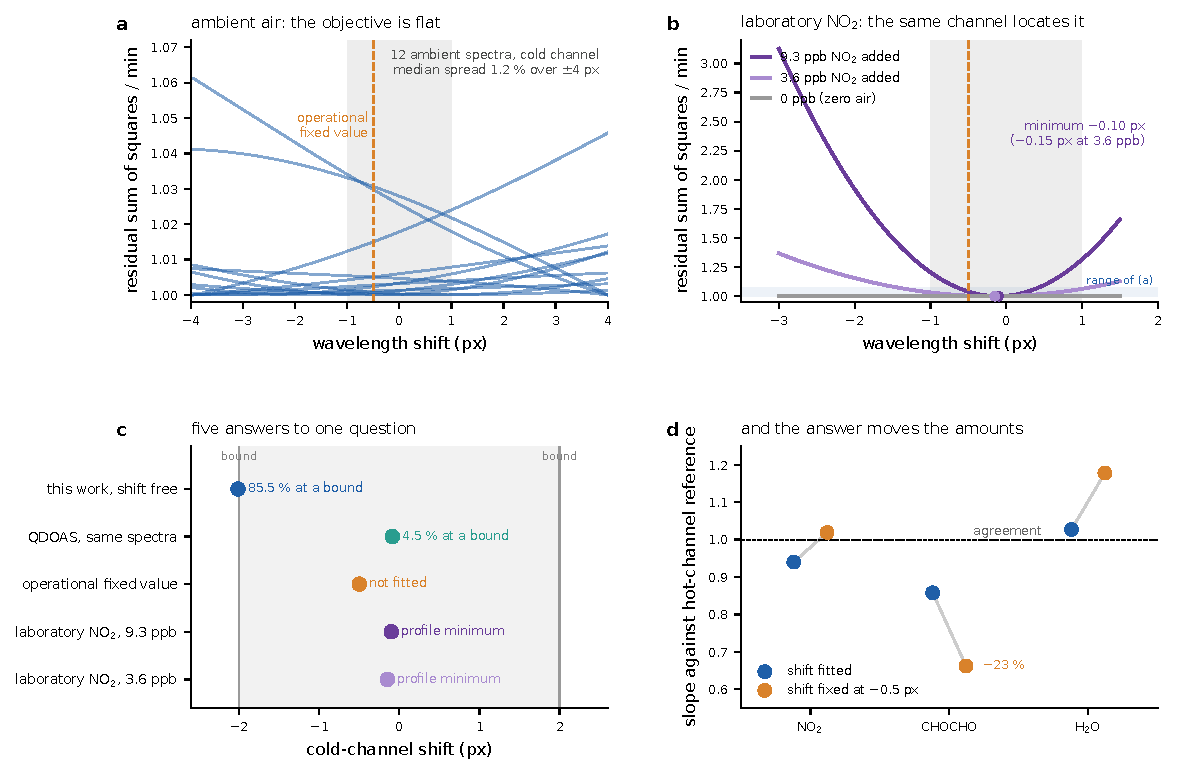
\includegraphics[width=\textwidth]{figures/fig05.pdf}
\caption{Identifiability of the cold-channel wavelength shift. \textbf{(a)} Profiled residual sum of squares against
shift for twelve ambient spectra, each normalised to its minimum; shaded, the range the operational configuration
allows; dashed, the value it fixes. \textbf{(b)} The same scan for the laboratory spectra of 2 June (zero air with 9.3
and 3.6\,ppb NO$_2$ added, and zero air alone); band, the vertical range of (a). \textbf{(c)} Shift returned for the
ambient spectra by two implementations under matched settings (with the fraction of fits at a bound), the operational
fixed value and the profile minima of (b). \textbf{(d)} Regression slope between the cold-channel retrievals of Augur
and QDOAS on the same spectra ($n = \fieldnum{5364}$), with Augur's shift fitted and fixed.}
\label{fig:5}
\end{figure*}

The budget of Sect.~\ref{sec:4} is not an artefact of basin hopping in the shift, and the reflectivity term hardly couples to
the shift at all (Appendix~\ref{app:D}, Table~\ref{tab:shift_degeneracy}).

Reporting \fieldnum{$-2.014 \pm 0.03$}\,px for a quantity the data locate only to \fieldnum{$\pm 2$}\,px is the failure described here, and
for this channel the resulting term is larger than any in Table~\ref{tab:2}. The ratio of the objective at the returned
value to that at a fixed reference point, which the fit evaluates anyway, would flag it (Sect.~\ref{sec:6.1}). Because
the shift belongs to the spectrograph rather than to the air, it could also be fitted jointly across the spectra of a
calibration block, as a separable problem with common nonlinear parameters. This is not implemented here and would
need an absorber in the block, as in the laboratory spectrum of Fig.~\ref{fig:5}b.

\subsection{Termination at a bound is a routine outcome}
\label{sec:5.2}

In this instrument bound termination is the normal state of one channel and a systematic response to perturbation in
another. The operational configuration (Appendix~\ref{app:A}) bounds the shift to $[-10, +0.5]$\,px in hot ANs and
$[-5, +5]$\,px in hot PNs and fixes it at $-0.5$\,px in the cold channel. In a sensitivity run that instead bounded the
cold shift to $[-1, +1]$\,px, every one of the \fieldnum{22} base fits returned exactly \fieldnum{$-1.000$}\,px, the bound itself, and was
reported as converged. In the production propagation of Sect.~\ref{sec:4} the cold shift is held fixed, as in operation,
and moves by exactly zero in every record, which confirms the configuration but also means the channel contributes
no information about the parameter.

On the clock-aligned basis of Table~\ref{tab:2}, \fieldnum{187} of the \fieldnum{9034} $\Sigma$ANs records are excluded because a fit of
either channel, unperturbed or perturbed, terminated at a bound. The split by perturbation was recorded only for the
earlier run on the unaligned reference: there, in hot PNs, the zero-air perturbation accounted for \fieldnum{121}
bound-terminated records against \fieldnum{4} for the unperturbed fits (the categories overlap), and the hot ANs channel had
none. In that run the operational fit was well inside its feasible region and the structural perturbation drove it
out, so the margin between the operational solution and the edge of identifiability is smaller than the size of a
reference error. Augur computes the termination states internally; the delivered campaign product did not carry them,
and the current version exports them as separate columns (Sects.~\ref{sec:2.6} and \ref{sec:6.1}).

\subsection{How far a record is from its calibration}
\label{sec:5.3}

The distance in time from a record to the calibration knots that produced its references varies over the campaign by
more than an order of magnitude, and the pipeline computes it in order to interpolate and then discards it. The
retrieval interpolates the reflectivity across an \fieldnum{11.8}\,h gap exactly as across a one-hour gap and returns the same
uncertainty in both cases. Coverage was measured over the whole campaign from calibration blocks extracted directly from the raw files,
independently of the retrieval. The extraction reproduces the production knot cache (\fieldnum{157}/\fieldnum{157} hot and
\fieldnum{164}/\fieldnum{164} cold knots at 0.000000\,s) and the alpha header's own \texttt{ZA\_count=}\fieldnum{1313}. Two distinct
deficits appear: records outside the knot range, and records inside a knot gap longer than two hours
(Table~\ref{tab:coverage}).

\begin{table}[t]
\caption{Calibration coverage of the retrieved records, from calibration blocks extracted directly from the raw files: number of records $n$; percentage of records outside the knot range and inside a knot gap longer than 2\,h (counts from the coverage
extractor; the retrieval itself has \fieldnum{9149} ambient records per heated channel in the budget window), for the zero-air ($I_0$) and reflectivity ($R$) references; and the longest reflectivity gap.}
\label{tab:coverage}
\small\setlength{\tabcolsep}{3pt}
\begin{tabular}{llllllll}
\tophline
instrument & window & $n$ & $I_0$ out of range & $I_0$ gap $>2$\,h & $R$ out of range & $R$ gap $>2$\,h & worst $R$ gap \\
\middlehline
hot ch1/ch2 & campaign & \fieldnum{76\,282} & \fieldnum{0.08}\,\% & \fieldnum{0.07}\,\% & \fieldnum{3.76}\,\% & \fieldnum{1.23}\,\% & \fieldnum{10.6}\,h \\
hot ch1/ch2 & budget window 05-18..24 & \fieldnum{9\,088} & \fieldnum{0.01}\,\% & \fieldnum{0.00}\,\% & \fieldnum{0.00}\,\% & \fieldnum{0.00}\,\% & \fieldnum{1.3}\,h \\
cold & campaign & \fieldnum{43\,259} & \fieldnum{0.13}\,\% & \fieldnum{0.34}\,\% & \fieldnum{2.89}\,\% & \fieldnum{11.03}\,\% & \fieldnum{11.8}\,h \\
cold & cold window 06-10..16 & \fieldnum{7\,069} & \fieldnum{0.42}\,\% & \fieldnum{0.00}\,\% & \fieldnum{17.32}\,\% & \fieldnum{18.31}\,\% & \fieldnum{11.8}\,h \\
\bottomhline
\end{tabular}
\end{table}

For the zero-air reference the interpolation is genuine: \fieldnum{0.08}\,\% of hot records lie outside the knot range and
\fieldnum{0.07}\,\% inside a gap longer than two hours, with the nearest knot a median \fieldnum{922}\,s away. The zero-air knot set is on
the corrected time axis -- the production cache over 05-18..24 reproduces a re-extraction at 0.000000\,s -- so the
$I_0$ column is unaffected by the displacement of Sect.~\ref{sec:5.4}.

The cold channel's deficit is a gap problem. The existing quality gates reject \fieldnum{11.3}\,\% of cold pairs against
\fieldnum{0.24}\,\% of hot pairs (\fieldnum{3} of \fieldnum{1\,264}); an independent count gives \fieldnum{75} of \fieldnum{743}, \fieldnum{10.1}\,\%, and nothing below turns on
the difference. Independent rejection at the \fieldnum{11.3}\,\% rate would leave \fieldnum{3.5}\,\% of cold records in gaps longer than two
hours, against the \fieldnum{11.03}\,\% observed. The worst gap, \fieldnum{11.8}\,h, is eleven consecutive rejected pairs, a run expected
0.03 times in the campaign even at a 40\,\% independent rejection rate. The rejections arrive in runs,
the episodic structure that Sect.~\ref{sec:6.1a} finds in the reflectivity variance itself. The same failures are absent
from the budget population (Sect.~\ref{sec:4.4}). In the cold channel, eleven of the thirteen zero-air blocks
identified as defective in Sect.~\ref{sec:6.3} fall outside the case set, because no reflectivity knot exists within
\fieldnum{2.8}--\fieldnum{5.8}\,h of them. A collapse of the zero-air signal takes the He/zero-air pair down with it, so
the two reference failures are one event seen twice. The interpolation already holds the time to the nearest knot, the length of the enclosing interval and whether a
record is out of range. Reported, they would separate the \fieldnum{0.00}\,\% of the budget window from the \fieldnum{18.31}\,\% of the cold
window, which no field in the current product distinguishes (Sect.~\ref{sec:6.1}).

\subsection{A reference error the fit does not see}
\label{sec:5.4}

The operational reflectivity reference was not clock-aligned. Its knots for 2026-05-18 to 05-30 lie on a time axis
that a later correction to the raw-data reader superseded, while the spectra lie on the corrected one. Every record in
that span, including the budget window of Sect.~\ref{sec:4}, was therefore retrieved with a reflectivity displaced by
nine hours. The zero-air reference is unaffected, because its knots were already on the corrected axis (verified to
0.000000\,s), and so is the cold channel, to which the correction does not apply. The retrieval was run twice over all
\fieldnum{9\,132} records of the window common to both heated channels, changing nothing but the knot time base
(Table~\ref{tab:clock_displacement}).

\begin{table}[t]
\caption{Change in the retrieved amounts when the heated channels are retrieved with the clock-aligned instead of the nine-hour-displaced reflectivity knots, over the records of the budget window: robust scale (rSD) and standard deviation (SD) of the change (ppb), and the rSD of the change relative to the rSD of the $R$ term in Table~\ref{tab:2}. $\Sigma$ANs is formed with $g' = \fieldnum{0.9524}$ as in Table~\ref{tab:2}.}
\label{tab:clock_displacement}
\begin{tabular}{llll}
\tophline
series & delta rSD (ppb) & delta SD (ppb) & vs the $R$ term of Table~\ref{tab:2} \\
\middlehline
ANs channel & \fieldnum{0.1048} & \fieldnum{0.1627} & \fieldnum{3.0} \\
PNs channel & \fieldnum{0.0358} & \fieldnum{0.0563} & \fieldnum{2.8} \\
$\Sigma$ANs & \fieldnum{0.100} & \fieldnum{0.1418} & \fieldnum{3.7} \\
\bottomhline
\end{tabular}
\end{table}

The displacement moves the alkyl nitrate product by \fieldnum{0.100}\,ppb, between three and four times the reflectivity term of
the budget and \fieldnum{1.44} times the whole of it. It is the largest term we can quantify within the retrieval; the
multiplicative scale discrepancy of Sect.~\ref{sec:3.6} is larger but lies outside it. It is not in Table~\ref{tab:2},
which measures what a reference's own uncertainty costs rather than what using the wrong reference costs.

\begin{table}[t]
\caption{What the fit report shows for the displacement of Table~\ref{tab:clock_displacement}: RMS change of the extinction spectrum (cm$^{-1}$), ratio of the residual and of the reported $\sigma$ between the two retrievals, change in the retrieved amount in units of the reported $\sigma$, and change in the fitted shift.}
\label{tab:clock_fitreport}
\begin{tabular}{llllll}
\tophline
 & $\alpha$ RMS change & residual ratio & reported $\sigma$ ratio & $|\delta c| / \sigma$ & $|\delta\,\mathrm{shift}|$ \\
\middlehline
ANs & $\fieldnum{3.37\times10^{-9}}$ & \fieldnum{1.0020} & \fieldnum{1.0022} & \fieldnum{1.99} & \fieldnum{0.0053}\,px \\
PNs & $\fieldnum{1.53\times10^{-8}}$ & \fieldnum{1.0016} & \fieldnum{1.0016} & \fieldnum{0.55} & \fieldnum{0.0065}\,px \\
\bottomhline
\end{tabular}
\end{table}

The fit report does not register the displacement (Table~\ref{tab:clock_fitreport}). The extinction spectrum changes by
an amount comparable to the single-scan noise floor of $\fieldnum{6.16\times10^{-9}}$, and the residual and the reported
uncertainty change by the same two parts in a thousand. The agreement is expected, because the reported uncertainty is a near-constant multiple of the residual RMS
(Sect.~\ref{sec:7.3}); an unchanged residual and an unchanged uncertainty are one witness reported twice. The fitted wavelength shift moves by \fieldnum{0.005}\,px, where the reference perturbations of
Table~\ref{tab:2} move it by \fieldnum{0.243}\,px (median), about forty times more, so the error is neither absorbed by the
nonlinear parameters nor revealed by the residual. The retrieved concentration of the 300\,$^{\circ}$C channel moves by two
reported standard deviations while every quality indicator in the fit report stays the same.

Correcting the time base changed the budget in both directions. The robust scale of the $\Sigma$ANs budget fell by
\fieldnum{7.0}\,\% (\fieldnum{0.0745} to \fieldnum{0.0693}\,ppb) while its standard deviation rose by \fieldnum{4.5}\,\% (\fieldnum{0.1183} to \fieldnum{0.1236}). The total
uncertainty relative to what is reported therefore widened at both ends, from \fieldnum{1.70}--\fieldnum{2.41} to \fieldnum{1.63}--\fieldnum{2.50}
times the same fit-reported sigma (Sect.~\ref{sec:4.4}). Coverage improved, from \fieldnum{8505} to \fieldnum{9034} of the window's \fieldnum{9149}
ambient records (\fieldnum{93.0} to \fieldnum{98.7}\,\%), because the misaligned knots had been falling outside the one-hour window that
admits a record to the perturbation experiment. The correlation between the two channels' joint responses fell from
\fieldnum{$+0.412$} to \fieldnum{$+0.146$}: because $\Sigma$ANs is a channel difference, a common-mode error partly cancels in it, and the
pre-correction cancellation was an artefact of an error the two channels shared. Both effects were properties of the
contaminated product, and the budget measured on it inherited them.

The cost of the displacement depends on how fast the reflectivity was moving. Across the boundary where the clock was
corrected, the affected side gives \fieldnum{0.0622}\,ppb against \fieldnum{0.0000}\,ppb on the unaffected side, which confirms that the
realignment touched only the intended knots. The displacement thus costs less near the boundary than in the budget
window, where the reflectivity moved fastest. The budget-window figure of \fieldnum{0.100}\,ppb is the value to quote;
\fieldnum{0.0622}\,ppb is range information, not a worst case.

The underlying cause was a stale derived file. The heated-channel clock itself ran on local time until 29 May and was
corrected in the reader after comparison with an external time reference. The reflectivity file was
written on 2026-07-10, the correction that invalidated it was committed on 2026-09-19, and the retrieval read both
without comparing them. Recording, for each derived reference, the version of the code and the raw files it was built
from detects this condition mechanically (Sect.~\ref{sec:6.1}); it is the only failure in this paper that admits a
complete remedy rather than a better report.

%% Sect. 6 -- from augur_AMT_§6 draft v1 (2026-09-20, later revisions to 2026-09-27)
%% The draft's "6.1a" is typeset as subsubsection 6.1.1 (label sec:6.1a).
\section{What should be reported, and what should be changed}
\label{sec:6}

Section~\ref{sec:4} established that the fit-reported uncertainty omits terms that are
several times larger than itself, and Sect.~\ref{sec:5} that convergence does not
imply identifiability. Neither finding requires a new retrieval algorithm to
act on. This section states what a DOAS product should carry instead of a
single uncertainty, and what in the measurement schedule is worth changing.
Of the four recommendations, two are implemented in Augur and evaluated against
the campaign: the knot gate (Sect.~\ref{sec:6.3}) and the coverage fields
(Sect.~\ref{sec:6.4}). The reporting convention of Sect.~\ref{sec:6.1} is implemented in
part -- the termination state, the distance to the nearest knot and the identity of
the reference file are exported, while the build time and time convention of each
reference are specified for implementation -- and the question of block length in
Sect.~\ref{sec:6.2} is left open by the measurements reported here. Section~\ref{sec:6.5} names the errors that none
of these measures reaches.

\subsection{Three numbers per retrieval, not one}
\label{sec:6.1}

Every retrieved amount is reported with
\begin{enumerate}
\item the \strong{fit uncertainty}, from the covariance of the projected problem
   (Sect.~\ref{sec:2.5}) -- what the residual supports, and nothing more;
\item the \strong{structural term}, evaluated for that scan's own calibration
   context rather than as a campaign constant; and
\item a \strong{context flag} recording the state of the references the scan depends
   on, in the specific form set out below.
\end{enumerate}

The third item is the one that has to be specified rather than gestured at,
because its value is entirely in which fields it carries. We report, per
record and per reference type (zero air, reflectivity), the fields of Table~\ref{tab:context_fields}.

\begin{table}[t]
\caption{Fields of the context flag, reported per record and per reference type (zero air, reflectivity), and the reason for each.}
\label{tab:context_fields}
\begin{tabular}{>{\raggedright\arraybackslash}p{0.38\textwidth}p{0.55\textwidth}}
\tophline
field & why \\
\middlehline
seconds to the nearest knot, with the side (before/after) & the side distinguishes interpolation from extrapolation \\
length of the bracketing interval & an eleven-hour gap and a fifteen-minute one are not the same interpolation \\
in-range flag & extrapolation is a different operation and should be nameable in a filter \\
number of adjacent calibration blocks rejected by the quality gates & the gates' cost, which Sect.~\ref{sec:6.4} argues must be reported wherever the gates are applied \\
identifier of the reference file, and when it was built & two products made from different calibration vintages are not comparable \\
the time convention the reference was built under & a correction applied upstream makes every earlier derived product stale \\
\bottomhline
\end{tabular}
\end{table}

The last field is there because of Sect.~\ref{sec:5.4}, and it is worth being exact about
what it would and would not have caught. The heated-channel clock ran on local time until 29 May
and on UTC thereafter, so for twelve days of the campaign the raw time stamps were nine hours off the
convention of the time axis; that is a property of the raw record, and no
provenance field detects it. It was detected the way such things are detected
-- against an external time reference -- and a correction was added to the
raw-data reader two months after the deployment ended.

What the field catches is the failure that followed. The reflectivity knots
had been computed before the correction existed, and nothing rebuilt them
afterwards. From that moment the retrieval was combining spectra on the
corrected time axis with a reference on the superseded one, and the twelve
days of product made from that combination are wrong by more than their whole
structural budget. This is not a clock problem; it is a staleness problem, and
it is general. Any correction applied upstream invalidates every derived
product built before it, and a pipeline in which derived products do not
record the convention they were built under cannot tell that it has happened.

The mismatch was not silent in the data. It surfaced as a nine-hour run of
out-of-range records at the very start of the deployment -- the first
zero-air block at 02:42, the first reflectivity knot at 11:40 -- and \fieldnum{42.3}\,\% of
that day extrapolated. The distance and in-range fields would have
carried that anomaly into the product on the first run after the correction,
rather than two months later. They would not have explained it: identifying
the cause needed the build time of the reflectivity file and the convention it
was built under. Detection and diagnosis are separate functions and need
separate fields.

There is also a cheaper protection than reporting, and it belongs in the same
subsection because it is the same information used earlier. A reference
carrying a time-convention tag can be checked against the tag on the spectra
at load time, and a mismatch refused rather than reported. Reporting turns a
silent error into a visible one; an assertion prevents it. We recommend the
assertion where the tags exist and the report in every case, because the
report is also what makes the error interpretable a year later, when the
person reading the product is not the person who ran it.

The second of these cannot be obtained cheaply, and it is worth saying why.
The amplification factor $I_0/(I_0-I)$, which governs how an error in the
zero-air reference enters the extinction, varies by a factor of forty between
records and is available without any fitting; it is a natural candidate for a
closed-form structural term. It does not work. Regressed against the measured
response it explains between \fieldnum{0.0}\,\% and \fieldnum{9}\,\% of the variance, with the wrong
sign, because the polynomial background absorbs the smooth part of the
perturbation and what reaches the gas columns is set by shape rather than
amplitude. Normalising the response by the retrieved amount does not help
either: the robust coefficient of variation is \fieldnum{0.80}--\fieldnum{1.09} in relative terms
against \fieldnum{0.83}--\fieldnum{1.11} in absolute. The structural term has to be obtained by
running the perturbation. That is available in post-processing and not in a
real-time monitor, and the two implementations differ accordingly.

The second and third exist because the first is conditional. A fit
uncertainty is a statement about the residual of a model assumed correct; it
is not a statement about the inputs to that model. Separating the three keeps
that distinction visible to whoever uses the product, instead of resolving it
silently into one number that is too small.

\subsubsection{Which remedy a term needs is readable from its shape}
\label{sec:6.1a}

The three structural terms call for three different actions, and the shape
statistic $s$ of Sect.~\ref{sec:4.3} says which. A term with $s \approx 1$ is Gaussian: its
error is spread evenly over all records and can only be reduced by a better
model. A term with $s \approx 0.7$--1 is dominated by measurement noise on the
references and responds to averaging. A term with $s \ll 0.7$ is concentrated
in a few records, where averaging is useless and detection is everything.

This is not an interpretation of $s$ but a prediction from it, and it can be
checked. Ordering the \fieldnum{155} hours of the budget window by their contribution to each term's variance gives Table~\ref{tab:shape_remedy}.

\begin{table}[t]
\caption{Concentration in time of each structural term over the hours of the budget window (clock-aligned basis of Table~\ref{tab:2}): shape statistic $s$; number (and fraction) of hours holding 90\,\% of the term's variance; the number of contiguous runs those hours form, with the number expected for the same count of hours drawn at random; share of the variance on the standard-deviation basis; and the remedy the shape indicates.}
\label{tab:shape_remedy}
\begin{tabular}{ll>{\raggedright\arraybackslash}p{0.17\textwidth}p{0.17\textwidth}p{0.12\textwidth}p{0.25\textwidth}}
\tophline
term & $s$ & hours holding 90\,\% of the variance & contiguous runs (random expectation) & share of variance (SD) & remedy \\
\middlehline
$I_0$ & \fieldnum{0.73} & \fieldnum{63} (\fieldnum{41}\,\%) & \fieldnum{24} (\fieldnum{38}) & \fieldnum{45}\,\% & longer calibration blocks (untested, Sect.~\ref{sec:6.2}) \\
$R$ & \textbf{\fieldnum{0.32}} & \textbf{\fieldnum{26} (\fieldnum{17}\,\%)} & \textbf{\fieldnum{12} (\fieldnum{22})} & \textbf{\fieldnum{52}\,\%} & detect and flag intervals (Sect.~\ref{sec:6.3}) \\
etalon $f$ & \fieldnum{0.98} & \fieldnum{118} (\fieldnum{76}\,\%) & \fieldnum{26} (\fieldnum{29}) & \fieldnum{3}\,\% & fit $f$ per scan, or model it \\
\bottomhline
\end{tabular}
\end{table}

The ordering by $s$ is the ordering by concentration, and the two-hour
interval from 23:00 UTC on 18 May to 01:00 UTC on 19 May alone holds \fieldnum{37}\,\% of the reflectivity term's variance.
The contiguous-run counts separate concentration from clumping: the
reflectivity hours form far fewer runs than the same number of hours drawn at
random, so they are episodes rather than scattered outliers and a flag can
address them. The etalon hours are indistinguishable from random, which is
the signature of a term no flag will help.

Read on the robust scale the ordering of the first two reverses -- $I_0$
carries \fieldnum{74}\,\% of the single-term quadrature sum and $R$ only \fieldnum{17}\,\% -- which is why the two scales
are reported side by side in Table~\ref{tab:2}. A term that is small for a typical
record and largest in total is exactly the one a campaign-mean uncertainty
hides.

\subsection{Calibration blocks: interval length and scans per block}
\label{sec:6.2}

The natural response to an interpolation error is to interpolate over shorter
intervals. How much that buys depends on the channel. Tripling the reflectivity interval from 2 to 6\,h was
measured to increase the interpolation error from \fieldnum{0.87}\,\% to \fieldnum{1.00}\,\% in hot PNs and from \fieldnum{2.05}\,\% to
\fieldnum{2.73}\,\% in hot ANs. In the 180\,$^{\circ}$C channel the error is set mostly by the noise on the knots, and a
shorter interval would buy little; in the 300\,$^{\circ}$C channel the interval carries curvature (Table~\ref{tab:splithalf_loo}),
and shorter intervals would help.

The other lever is the number of scans averaged into each calibration block, and the evidence on it is not
conclusive (Appendix~\ref{app:C}). Within the operational block ($N = 34$ scans, $T = 32$\,s), doubling the number of
scans averaged reduces the scatter of contiguous sub-blocks by \fieldnum{7}\,\% in the ANs channel, against the 29\,\% that
independent scans would give; but the range that can be measured this way lies entirely below the operational block
length, so it is mildly unfavourable rather than decisive, and the measurement that would settle it -- operating one
longer block -- has not been made. Even with white averaging the return would be modest: the zero-air term carries
\fieldnum{45}\,\% of the $\Sigma$ANs variance, so a fourfold block, which would raise the calibration duty from 1.20 to 3.89\,\%,
would lower the structural budget from \fieldnum{0.1236} to \fieldnum{0.1008}\,ppb (\fieldnum{18.5}\,\%), whereas flagging the few
defective reflectivity intervals would lower it to \fieldnum{0.0901}\,ppb. That ordering -- flagging before averaging --
holds whatever the block scaling turns out to be, because the reflectivity term is concentrated in a few episodes and
the zero-air term is not (Sect.~\ref{sec:6.1a}).

\subsection{Gating defective knots}
\label{sec:6.3}

Not all calibration blocks are usable, and the bad ones are few. Ordering the
cold-channel zero-air blocks by their leave-one-out influence, the worst
single block carries \fieldnum{28}\,\% of the total variance, the worst three carry \fieldnum{76}\,\%,
and the worst five carry \fieldnum{97}\,\%. A structural term computed over all blocks is
therefore a statement about a handful of them.

They are identifiable before any fit is attempted. A single observable -- the
block's light level relative to the campaign median -- with the threshold
$I/\tilde{I} < 0.5$ selects \fieldnum{13} of the \fieldnum{38} blocks whose influence exceeds 2\,\%,
but those \fieldnum{13} include nine of the worst ten and account for \fieldnum{99.9}\,\% of the
influence variance. The \fieldnum{25} blocks it misses are all in the \fieldnum{2}--\fieldnum{3}\,\% range. The
threshold excludes \fieldnum{8}\,\% of blocks.

Classification accuracy is the wrong figure of merit here and would have
rejected this threshold: \fieldnum{13} of \fieldnum{38} is a poor hit rate and a good filter. What
matters is the variance removed, and a single observable removes essentially
all of it. No multi-indicator scheme is needed.

The asymmetry with the reflectivity is worth recording, because it explains why
only one of the two references needed this. Reflectivity knots already pass
three quality gates -- a minimum fraction of valid pixels, an acceptance band on
the retrieved effective path length, and limits on the calibration residual --
so a defective helium or zero-air pair is rejected before it becomes a knot.
The zero-air reference had no equivalent: every block became a knot regardless
of how much light reached the detector. The gate described here closes that
gap. It is implemented with the threshold expressed as a fraction of the run's
own median block intensity rather than as an absolute count, so it transfers
between instruments, and it is disabled by default so that reprocessing an
existing product is an explicit choice rather than a silent change.

\subsection{Coverage: say when the reference is far away}
\label{sec:6.4}

Two things are missing, and conflating them produces the wrong prescription.
One is \emph{extrapolation}: records outside the range spanned by the reflectivity
knots. The other is a \emph{gap}: records between two knots more than two hours
apart. The hot channel has \fieldnum{3.76}\,\% of the first and \fieldnum{1.23}\,\% of the second over
the campaign; the cold channel \fieldnum{2.89}\,\% and \fieldnum{11.03}\,\%. Zero air has neither
(\fieldnum{0.08}\,\% and \fieldnum{0.07}\,\%), so the constraint is entirely on the reflectivity.

Two causes lie behind the deficit that survives clock alignment, and they cost different things to remove. The first
is bookkeeping and the cheapest fix in this paper: reflectivity generation stopped at 07-09, which produces the hot
channel's trailing extrapolation and is removed by re-running over files that already exist. The second is clustered
rejection of calibration pairs, \fieldnum{11.3}\,\% of cold pairs, which explains the cold gaps (\fieldnum{11.03}\,\% over the campaign and
\fieldnum{18.31}\,\% in the cold window); its remedy is to restore the light level or, failing that, redundancy. Only this
second cause is about how often the instrument calibrates, and even there the average rate is not the problem.
Independent rejection at the measured rate would leave \fieldnum{3.5}\,\% of cold records in gaps longer than two hours,
against \fieldnum{11.03}\,\% observed. The rejections arrive in runs: the worst cold gap, \fieldnum{11.8}\,h, is eleven consecutive
rejected pairs, which even at a 40\,\% independent rejection rate would be expected 0.03 times in the campaign. This
is the episodic structure Sect.~\ref{sec:6.1a} found in the reflectivity variance itself -- \fieldnum{26} of \fieldnum{155} hours carrying
90\,\% of it, in \fieldnum{12} contiguous runs where \fieldnum{22} would be expected at random -- seen from the calibration side.

It also locates the cost of quality control. The three gates the reflectivity already passes cost the hot channel
\fieldnum{0.24}\,\% of its pairs and the cold channel \fieldnum{11.3}\,\%; in the cold channel the gates are, correctly, the proximate
cause of the coverage deficit. This cuts against the argument of Sect.~\ref{sec:6.3}, which asks for a gate that zero
air does not yet have: gates remove variance and they remove coverage, and a pipeline that gates without also
reporting what the gating cost has moved the error somewhere it is harder to see. The context flag of
Sect.~\ref{sec:6.1} closes that loop. The same caution applies to the budget: the reflectivity contribution of
Sect.~\ref{sec:4} is measured by removing a knot and re-interpolating, so its magnitude scales with how far apart the
knots already are, and a sparse reference presents itself as a dominant term partly because it is sparse -- which is
why the remedy belongs to the schedule and to reprocessing rather than to the retrieval. Records in gaps are not
covered by the budget at all, since a perturbation experiment needs a knot to perturb; they are reported with the
context flag set and excluded from any statistic that assumes a characterised uncertainty.

In the heated channels zero air is measured every hour and helium every three, and each reflectivity knot pairs a
zero-air block with the most recent helium block that passed the quality gates (Appendix~\ref{app:A},
Table~\ref{tab:cal_schedule}), so the knots are hourly while their helium half is up to three hours old, and older when a
helium block is rejected. A rejected zero-air/helium pair removes one hourly knot and leaves a two-hour gap; a rejected
helium block removes no knot but makes the following knots use helium measured up to six hours earlier. Matching the
helium cadence to the zero-air cadence would bring the total calibration duty from 1.20\,\% to 1.79\,\% and make the
helium half of every knot contemporaneous. Whether it would also shorten the gaps depends on why pairs are rejected,
which in the cold channel is mainly the light level. The case for it is redundancy against runs of rejection and
contemporaneity, not precision: in the 180\,$^{\circ}$C channel the reflectivity error depends only weakly on interval
length (Sect.~\ref{sec:6.2}), so more frequent helium would not make a well-covered record much more accurate. At
1.2\,\% of the measurement time, calibration is the binding constraint on none of these remedies.

\subsection{Errors that neither the fit report nor the proposed fields detect}
\label{sec:6.5}

The convention of Sect.~\ref{sec:6.1} makes visible what the pipeline already knows. It cannot make visible what the
pipeline does not know, and two such errors appear in this record.

The first is a multiplicative gain error. Against a co-located NIER analyser the heated-channel NO$_2$ reads low by a
factor of about \fieldnum{0.6} while the ambient-temperature channel agrees (Sect.~\ref{sec:3.6}). A gain leaves the residual, the
reported uncertainty, the termination state and every distance and provenance field unchanged, and the zero-air test
of Sect.~\ref{sec:7.2} is blind to it because a gain applied to zero is zero. Only a comparison with an independent
measurement of the same quantity -- a reference analyser, a cylinder, or a channel that should agree -- reveals it,
and such a comparison does not by itself identify the cause.

The second is the raw light level. All six ambient-temperature excursions of Sect.~\ref{sec:7.3} coincide with spectra
that fell below 30\,\% of their usual count at 460\,nm; the residual finds them, and the reference context is abnormal
in five of them, but none of the proposed fields names the cause. The light level of each spectrum, and the helium and
zero-air intensities of each calibration block rather than only their ratio, are known when they are recorded and
could travel with the product as further context; we have not evaluated them for the heated channels.

%% Sect. 7 -- from augur_AMT_§7 draft v1 (2026-09-22; Sect. 7.3 recounted 2026-09-27)
\section{Field demonstration}
\label{sec:7}

\subsection{Instrument and deployment}
\label{sec:7.1}

The retrieval is applied here to a thermal-dissociation broadband
cavity-enhanced absorption spectrometer with two heated and one ambient-temperature cavity, of the design described by \citet{Min_2016} and \citet{Nam_2022}. Ambient air is split between a cell held at
180\,$^{\circ}$C, in which peroxy nitrates dissociate, and one at 300\,$^{\circ}$C, in which alkyl
nitrates dissociate as well; a third cell at ambient temperature measures NO$_2$
directly. Each channel measures the extinction of the same cavity geometry,
$d = 51.8$\,cm with $R_L = 1.0$ (assumed, not measured; since $\alpha \propto R_L$ it enters as a
multiplicative factor), so the three differ in what has been converted
to NO$_2$ upstream rather than in how the spectrum is formed. The sums of peroxy
and alkyl nitrates follow as channel differences.

The instrument was deployed at Suncheon Shindae (SDD) from 2026-05-18 to
07-10 as part of a multi-institution intensive campaign. Zero-air blocks of 34
scans over 32\,s run hourly and helium blocks of the same specification every
three hours, a combined calibration duty cycle of 1.20\,\%. Spectra are
retrieved in 444.118--470.562\,nm with a third-order Chebyshev baseline for the
180\,$^{\circ}$C channel and 430--462\,nm with a fourth-order baseline for the 300\,$^{\circ}$C
channel; the ambient-temperature channel uses 438.420--475.741\,nm and a
fourth-order baseline. The dispersion is 0.0481\,nm\,px$^{-1}$ and the
instrument line shape of the heated channels has a full width at half maximum of 0.683\,nm (0.765--0.785\,nm in
the ambient-temperature channel, Sect.~\ref{sec:4.1}). The field numbers of this paper were checked against a
reprocessing with a corrected pressure-sensor pairing, which changes the channel NO$_2$ by $\pm$\fieldnum{0.25}\,\%, and are
reported as first computed.

The three channels also sit at different offsets from their wavelength
calibrations: the operational shift bounds are $-10$ to $0.5$\,px for the
300\,$^{\circ}$C channel and $-5$ to $5$\,px for the 180\,$^{\circ}$C channel; in the
ambient-temperature channel the shift is fixed at $-0.5$\,px and the squeeze at
its identity value, i.e. no stretch (Sect.~\ref{sec:5.1}). The median fitted shift in the 300\,$^{\circ}$C channel is \fieldnum{$-6.12$}\,px.

Only the properties the retrieval depends on are given here. The instrument
itself, its inlet and its conversion efficiencies are characterised elsewhere.

\subsection{Noise floor of the product record}
\label{sec:7.2}

The quantity the product reports is a channel difference, so its noise floor
has to be measured on the difference and not assembled from the channels. The
two hot channels share a light source, a cavity and a clock, and their
zero-air blocks coincide in time, so \fieldnum{155} blocks pair exactly and the
difference can be formed record by record (Table~\ref{tab:noise_floor}). Assembling the floor from the
channels in quadrature would assume an independence that there is no reason
to expect.

\begin{table}[t]
\caption{Noise floor of the $\Sigma$ANs product, measured on the paired zero-air blocks of the two heated channels: 1$\sigma$, 3$\sigma$ detection limit, median at a true zero, and the ratio of the measured 1$\sigma$ to the uncertainty column shipped with the product. Standard-deviation values are approximate, recombined from the channel values with $g' = \fieldnum{0.9524}$; robust-scale values are from the earlier evaluation with a channel factor of 0.82 and were not recomputed.}
\label{tab:noise_floor}
\begin{tabular}{lll}
\tophline
 & robust scale & standard deviation \\
\middlehline
measured 1$\sigma$ & \fieldnum{0.0676} & $\approx$\fieldnum{0.086}\,ppb \\
\textbf{detection limit, 3$\sigma$} & \textbf{\fieldnum{0.203}} & \textbf{$\approx$\fieldnum{0.257}\,ppb} \\
median value at a true zero & \fieldnum{$+0.0054$}\,ppb & \fieldnum{$+0.0054$}\,ppb \\
against the product-column \fieldnum{0.0806}\,ppb & \fieldnum{0.84} & $\approx$\fieldnum{1.06} \\
\bottomhline
\end{tabular}
\end{table}

The channels turn out to be nearly uncorrelated, $r = \fieldnum{-0.093}$, so the
quadrature assembly would have come within about \fieldnum{4}\,\% of the measured value. That
is a result of the measurement rather than a licence to skip it: the same
comparison on an instrument whose channels shared a drift would not be so
forgiving, and nothing in the fit report distinguishes the two cases.

The median at a true zero is \fieldnum{$+0.0054$}\,ppb, and it is the same at the channel
level and in the difference. A product assembled through zero-air
interpolation, a Rayleigh correction, a time-interpolated reflectivity, a
spectral fit and a channel subtraction returns zero when the truth is zero,
to a twentieth of its own detection limit. This closes the additive chain end to end
and belongs with the verification of Sect.~\ref{sec:3.1} as much as here; a zero test is blind to gain errors, such as
the scale discrepancy of Sect.~\ref{sec:3.6}.

Read against the uncertainty column shipped with the product, the product's noise floor is roughly covered:
\fieldnum{0.84} to about \fieldnum{1.06} times that column's \fieldnum{0.0806}\,ppb, depending on the scale. This is
not in tension with Sect.~\ref{sec:4}, and the distinction matters enough to state. What is
measured here is a zero-air floor -- the same references, minutes apart, no
atmosphere and no elapsed time for a reference to go stale. What Sect.~\ref{sec:4} measures
is what happens when a reference is wrong, and that is a different question
with a different answer: \fieldnum{1.32} to \fieldnum{1.83} times the same product-column figure of
\fieldnum{0.0806}\,ppb (Sect.~\ref{sec:4.4}). (Against the fit-propagated $\sigma$ of \fieldnum{0.0541}\,ppb, the denominator of
Sect.~\ref{sec:4.4}, the total is \fieldnum{1.63} to \fieldnum{2.50} times that value, and in \fieldnum{46.1}\,\% of the \fieldnum{8832} budget records
the structural change exceeds that record's own fit-propagated $\sigma$.) A reported uncertainty can describe the
photon noise of a product faithfully and still say nothing about the
references the product was built from.

The reported uncertainty column of the product is not the quadrature of the
channel columns -- it is \fieldnum{1.48} times larger, \fieldnum{0.0806}\,ppb against \fieldnum{0.0543} --
because it is not a measurement uncertainty. It is the inter-channel gain
systematic described in Sect.~\ref{sec:4.4}, which scales with the NO$_2$ amount, and for that
reason the ratios of Sect.~\ref{sec:4} are taken against the fit-propagated sigma rather than
against this column.

\subsection{The reporting convention in operation}
\label{sec:7.3}

Applied retrospectively to this deployment, in the heated and the ambient-temperature channels alike, the
quantities Sect.~\ref{sec:6.1} asks for separate what the fit report catches from what it does not
(Fig.~\ref{fig:6}); the provenance fields among them are specified, not yet implemented.

One episode is not caught by the fit report at all: the reference-convention
displacement of Sect.~\ref{sec:5.4}. From 18 to 30 May the heated channels were retrieved with
a reflectivity displaced by nine hours; the alkyl nitrate product moved by
\fieldnum{0.100}\,ppb while the residual and the reported uncertainty changed by two parts
in a thousand. Across the deployment the reported uncertainty of the ANs
channel is a near-constant multiple of the residual RMS ($r = \fieldnum{+0.999}$ over
all \fieldnum{74\,667} records; the ratio varies by \fieldnum{2.8}\,\% between its 5th and 95th
percentiles), so the two are one witness, not two. Among the proposed fields, the distance and in-range fields flag
these records (Sect.~\ref{sec:6.1}) and only the provenance fields would name the cause.

The ambient-temperature channel supplies the opposite case. Its six excursions
below $-5$\,ppb (\fieldnum{19} hourly medians between 19 May and 2 June) are all visible in
the fit itself: the residual RMS is \fieldnum{8} to \fieldnum{600} times its campaign median and the
reduced chi-square \fieldnum{5.6} to \fieldnum{91}, against \fieldnum{1.2} in ordinary hours. Five of the six
coincide with an abnormal reference context -- the bracketing reflectivity knots
are \fieldnum{2.6} to \fieldnum{9.0}\,h apart against 1\,h nominal, or one of them departs from its
running median by \fieldnum{66} to \fieldnum{300}\,\% against a typical \fieldnum{10}\,\% -- so the
distance-to-reference and knot-validity fields explain them, but are not needed
to find them. The sixth, four hours on 2 June, has an ordinary reference
context and is identified by the residual alone. All six share a proximate
cause that none of these fields names: the raw light level. In each, the
ambient or the zero-air spectrum, or both, fell below 30\,\% of its usual count
at 460\,nm, in four of them to within a few hundred counts of the detector dark
level; on 2 June only the ambient path lost light (\fieldnum{22}\,\% of the zero-air level),
which is why the reference stayed ordinary (Fig.~\ref{fig:6}). The misfit threshold ($\chi^2 > 1.5$) is itself
signal-dependent (Sect.~\ref{sec:4.1}); these excursions exceed it by an order of magnitude or more.

In the heated channels no hourly median falls below $-0.5$\,ppb over the
deployment. The termination-state field flags one episode: for eleven minutes
on 21 June the 180\,$^{\circ}$C channel returned its shift at the $+5$\,px bound, and the
residual is raised over the same records (reduced chi-square \fieldnum{4.7} to \fieldnum{5.5}). Here
the residual signals that something is wrong and the termination state says
what.

In each of these cases the fit either reports an ordinary residual and
uncertainty for a displaced amount, or reports an abnormal one without saying
why. For the displacement and for the bound episode, one of the context quantities -- distance to the
nearest reference, termination state, or reference provenance -- supplies what is missing. For the cold
excursions the proximate cause, the raw light level, is not among the proposed fields. And the heated-channel
NO$_2$ scale, low against the co-located NIER analyser by a factor of about \fieldnum{0.6} (Sect.~\ref{sec:3.6}), is invisible to
the fit report and to every proposed field. The fields narrow the gap between what a fit reports and what is
known about the record; they do not close it.

\begin{figure*}[p]
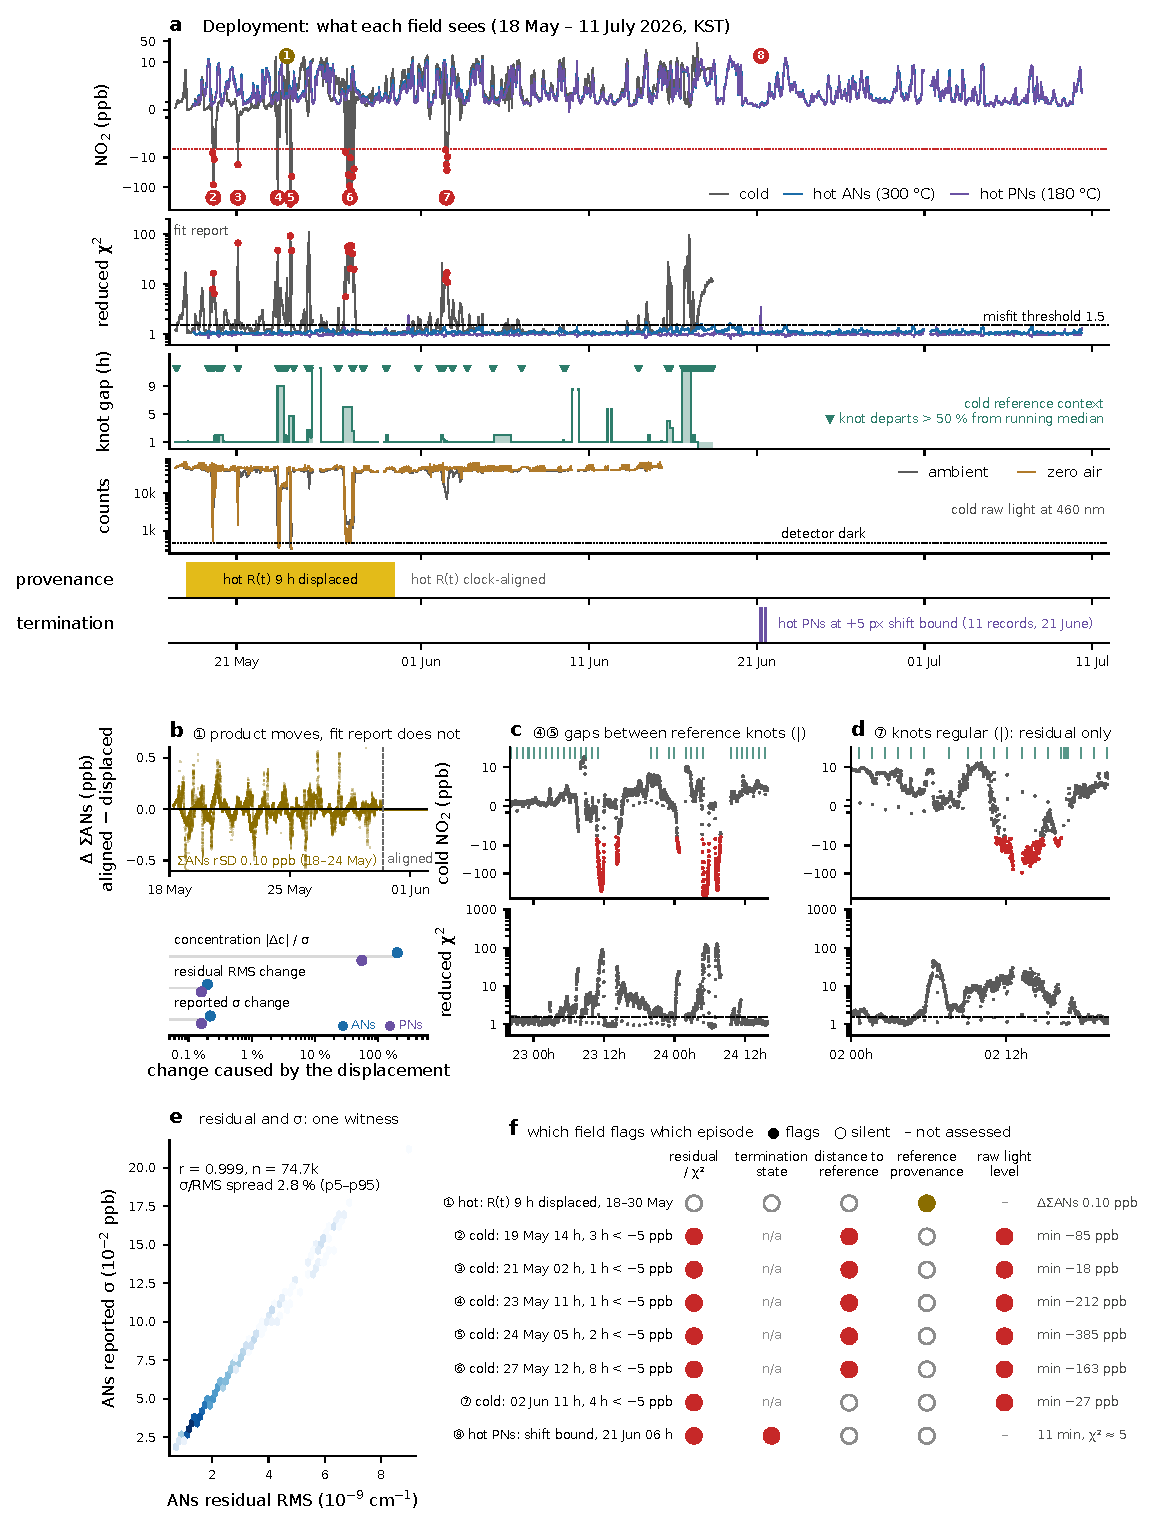
\includegraphics[width=\textwidth,height=0.62\textheight,keepaspectratio]{figures/fig06.pdf}
\caption{What each reporting field flags during the deployment (18 May -- 11 July 2026, KST).
\textbf{(a)} From top: hourly median NO$_2$ of the three configurations (symmetric-log axis; red: cold hours below
$-5$\,ppb); hourly median reduced $\chi^2$ with the misfit threshold of 1.5; for the cold channel, the interval between
the reflectivity knots that bracket each record (triangles: a knot departing by more than 50\,\% from its running
median); the raw cold-channel light at 460\,nm in ambient and zero-air spectra, with the detector dark level;
the provenance of the heated-channel reflectivity; and records that terminated at a shift bound.
Numbered badges mark the episodes of panel f. \textbf{(b)} Episode \textcircled{\scriptsize 1}: the change in $\Sigma$ANs when the heated channels are
retrieved with the clock-aligned instead of the 9\,h displaced reflectivity (points: records; line: 6\,h median;
dashed: end of the displaced span). Below, for 18--24 May, the change in concentration expressed in units of its
reported $\sigma$, against the change in residual RMS and in reported $\sigma$. \textbf{(c)} Episodes \textcircled{\scriptsize 4} and \textcircled{\scriptsize 5}: cold NO$_2$ and
reduced $\chi^2$ per record, with reflectivity knot times as ticks; the excursions fall in \fieldnum{9.0}\,h and \fieldnum{4.7}\,h gaps.
\textbf{(d)} Episode \textcircled{\scriptsize 7}: the same for 2 June, where the knots are regular and only the residual flags the records.
\textbf{(e)} Reported $\sigma$ against residual RMS for every hot ANs record. \textbf{(f)} For each episode, whether the residual
($\chi^2 > 1.5$), the termination state, the distance to the nearest reference (knot interval $>2$\,h or knot
departure $>50$\,\%), the reference provenance, or the raw light level (ambient or zero-air count below 30\,\% of its usual value) flags it;
the light level was not assessed for the heated channels (--); the cold configuration has fixed shift and squeeze, so its
termination state carries no bound information (n/a).}
\label{fig:6}
\end{figure*}

%% Sect. 8 -- from augur_AMT_§8 draft v1 (2026-09-22); rewritten for length and sentence length 2026-09-29.
\conclusions
\label{sec:8}

We have presented Augur, an open DOAS retrieval posed in the extinction domain as a separable nonlinear least-squares
problem and solved by variable projection. It is configured by instrument and campaign profiles, and its diagnostics
were demonstrated on one field case: a thermal-dissociation broadband cavity-enhanced absorption spectrometer with two
heated and one ambient-temperature cavity. The formulation is conventional; the implementation makes three things cheap: substituting a calibration reference
without reprocessing the campaign, evaluating the projected objective anywhere in the nonlinear parameters, and
carrying the termination state and the distance to each reference into the product.

The code solves the problem it states: synthetic recovery is at the level of the linear algebra, the analytic
Jacobian agrees with finite differences to round-off, and Augur and QDOAS agree on synthetic spectra. On field spectra they agree in NO$_2$ with
$r^2 \ge \fieldnum{0.990}$ but differ in the heated-channel scale by \fieldnum{4}--\fieldnum{6}\,\%. The full chain returns \fieldnum{$+0.0054$}\,ppb at a true zero, a
twentieth of the three-sigma detection limit of \fieldnum{0.203} to about \fieldnum{0.257}\,ppb, which tests the additive chain only.

The first question concerned errors the fit cannot see. With white noise and a complete model the reported sigma tracks
the synthetic scatter to within about ten per cent, rising to 1.32 with a free shift; against the calibration chain it
fails. For the channel-difference product, perturbing the
zero-air reference, the reflectivity and the etalon as the operational pipeline builds them gives, in the
best-calibrated week, a structural contribution of \fieldnum{1.28} (robust scale) to \fieldnum{2.29} (standard deviation) times the
reported sigma. The total uncertainty is \fieldnum{1.63} to \fieldnum{2.50} times what the fit reports for the same 60\,s records. None of the
calibration-chain terms enlarges the residual. These terms add to the campaign-constant cross-section and
Rayleigh uncertainties of earlier treatments rather than replacing them (Sect.~\ref{sec:4.6}). The magnitudes belong to
this instrument; the mechanism, an intermittently measured reference interpolated to every record, is general.

The second question concerned information the pipeline holds. With the cold shift bounded to $\pm 1$\,px in a
sensitivity run, every base fit of the ambient-temperature channel returned its shift at the bound. In the budget
propagation \fieldnum{187} of \fieldnum{9034} records were excluded because a fit terminated at a bound, and all were recorded as
converged. In one window the projected objective varies by
about one per cent across four pixels of shift, in another over five orders of magnitude, and both fits report
convergence. A reflectivity reference on a superseded time convention displaced the alkyl nitrates by \fieldnum{1.44} times the
structural budget, while the residual and the reported uncertainty moved by two parts in a thousand.

A third category lies outside both. Against a co-located NIER analyser the heated-channel NO$_2$ reads low by a factor of
about \fieldnum{0.6} while the ambient-temperature channel agrees. This multiplicative discrepancy, whose cause is unresolved, is
the largest error in the record, and neither the fit report nor the proposed fields see it (Sects.~\ref{sec:3.6} and
\ref{sec:6.5}).

We therefore propose that a retrieval report three numbers: the fit uncertainty, the structural term for the record's own
calibration context, and a context flag (Sect.~\ref{sec:6.1}). Every implementation already computes the flag's fields,
except the build time and time convention of a reference, which must be recorded when the reference is built.
Quality gates should be reported with the coverage they cost, because they remove coverage as well as variance
(Sect.~\ref{sec:6.4}). Where the interpolation error is set by knot noise, as in the 180\,$^{\circ}$C channel, averaging more scans per
calibration block is the lever to test; the within-block evidence is unfavourable and the decisive measurement has not
been made (Sect.~\ref{sec:6.2}).

The evidence is one instrument over one campaign. The code is not tied to that instrument (Appendix~\ref{app:A}), but
its behaviour on other configurations is not shown here. The reporting convention and the synthetic benchmark of 261
cases, which contains no retrieval code or field data, should carry beyond it; extending the benchmark across line
shapes, windows and pixel grids would separate what is general from what is ours.

Three extensions follow from the results. Fitting one shift jointly across the spectra of a calibration block
could remove the indeterminacy diagnosed here, given an absorber in the block (Sect.~\ref{sec:5.1}). Treating the zero-air
reference and the reflectivity as measured quantities with their own covariance would propagate the structural term
inside the fit (Sect.~\ref{sec:4.6}). And the raw light level of each spectrum, the proximate cause of all six ambient-temperature excursions, should travel
with the product together with the helium and zero-air intensities of each calibration block (Sect.~\ref{sec:6.5}).


%% Code and data availability -- from augur_AMT_availability draft (2026-09-27).
%% DOIs [TBD-Z1] (Augur release) and [TBD-Z2] (benchmark) are obtained just before submission.
\codedataavailability{Augur is free software released under the MIT licence. The version used in this
paper, v0.2.0, is archived at Zenodo (\url{https://doi.org/}[TBD-Z1]) and developed at
\url{https://github.com/HwanKyungLee/CAESAR}. The archive contains the analysis code, the
test suite referred to in Sect.~\ref{sec:3}, the scripts that produce the figures of this
paper, and derived calibration constants (wavelength-calibration polynomials,
instrument line-shape widths and instrument-convolved reference cross sections).
The original laboratory cross sections are not redistributed; they are available
from their providers: NO$_2$ \citep{Vandaele_2002}, CHOCHO \citep{Volkamer_2005}, O$_4$ \citep{Thalman_2013}, and H$_2$O line data from HITRAN \citep{Gordon_2022}.

The synthetic benchmark of Sect.~\ref{sec:3.4} -- 261 spectra with known truth, their
generator, the reference implementation and its scorecard -- contains no field data
and is archived separately (\url{https://doi.org/}[TBD-Z2]). Figure~\ref{fig:3} can be reproduced
from the two archives alone.

Raw instrument data and the field time series used in Sects.~\ref{sec:4} to \ref{sec:7} (60\,s
extinction spectra, zero-air and reflectivity knot tables, and retrieved NO$_2$
amounts, 18 May to 11 July 2026) are not publicly distributed; they are available
from the corresponding author on reasonable request.}


\appendix
%% Appendix B -- from augur_AMT_부록B draft v1 (2026-09-22). Synthetic / algebraic only: no \fieldnum.
%% Phase 3: typeset as Appendix B, between Appendix A (configuration) and Appendix C (calibration-block length).
\section{The projected Jacobian, column scaling and the joint covariance}
\label{app:B}

\subsection{Setup}
\label{app:B1}

Write the forward model of Sect.~\ref{sec:2.1} for one spectrum as
\begin{equation*}
\alpha \;=\; \Phi(\theta)\,c \;+\; \varepsilon ,
\end{equation*}
where $\theta = (\text{shift}, \text{squeeze})$ enters the columns of $\Phi$
through the resampling of the reference cross sections, and $c$ collects the
gas amounts and the Chebyshev baseline coefficients. The problem is separable:
for any $\theta$ the linear parameters are determined by least squares,
$c^\ast(\theta) = \Phi^{+}\alpha$, and the objective reduces to the \emph{profiled}
residual
\begin{equation*}
r(\theta) \;=\; \bigl(I - \Phi(\theta)\Phi(\theta)^{+}\bigr)\,\alpha
\;=\; P^{\perp}(\theta)\,\alpha .
\end{equation*}
The optimiser searches only $\theta$; $c$ is never a search direction. This is
variable projection \citep{Golub_1973}.

\subsection{The derivative has two terms}
\label{app:B2}

Differentiating the projector rather than the fit gives, for each nonlinear
parameter $\theta_j$ and with $\Phi_j = \partial\Phi/\partial\theta_j$,
\begin{equation*}
\frac{\partial r}{\partial \theta_j}
\;=\; -\Bigl[\, P^{\perp}\Phi_j\Phi^{+}
\;+\; \bigl(P^{\perp}\Phi_j\Phi^{+}\bigr)^{\!\top} \Bigr]\alpha .
\end{equation*}
The first term is the change in the residual caused by moving the column
space; the second is the change caused by the reprojection of $\alpha$ onto
it. \citet{Kaufman_1975} drops the second, which is cheaper and is often adequate
because it does not change the stationary point -- both expressions vanish
where the true gradient vanishes -- only the path taken to it and the
curvature reported there.

It is not adequate here. On a small separable problem with the same structure
as Sect.~\ref{sec:2.1} -- two Gaussian absorber columns and three Chebyshev columns -- the
two-term expression agrees with a central finite difference of $r(\theta)$ to
$2\times10^{-10}$ relative, while the one-term expression is in error by 20\,\%
and 17\,\% in the two nonlinear parameters. The step-size sweep of Sect.~\ref{sec:3.2} measures
the same thing on the real problem: the analytic derivative descends to the
round-off floor, which an expression missing a term of that size could not do.

\subsection{Column scaling changes nothing, until it changes everything}
\label{app:B3}

Replace $\Phi$ by $\Phi D$ for any invertible diagonal $D$. Then
$(\Phi D)^{+} = D^{-1}\Phi^{+}$, so $P = \Phi D D^{-1}\Phi^{+} = \Phi\Phi^{+}$
and $P^{\perp}$ are unchanged, and in the derivative of Appendix~\ref{app:B2} the factors
$D$ and $D^{-1}$ cancel term by term. The profiled residual, its derivative
and the fitted $\theta$ are therefore invariant under rescaling of the
columns; only $c$ and its covariance rescale, and they rescale exactly
inversely, so the retrieved amounts are unchanged.

That is the algebra. The arithmetic is not invariant, and the failure is
abrupt rather than gradual, because $\Phi^{+}$ is computed with a rank
tolerance (Table~\ref{tab:colscaling}).

\begin{table}[t]
\caption{Effect of rescaling one column of the small test problem of Appendix~\ref{app:B2} on the condition number $\kappa$, on the projector $P^{\perp}$ and on the derivative $\partial r/\partial\theta$.}
\label{tab:colscaling}
\begin{tabular}{llll}
\tophline
column scaling & $\kappa(\Phi D)$ & $\lVert\Delta P^{\perp}\rVert$ & relative change in $\partial r/\partial\theta$ \\
\middlehline
none & $9.3$ & $0$ & $0$ \\
$10^{-3}$ on one column & $6.1\times10^{5}$ & $2.4\times10^{-10}$ & $1.1\times10^{-10}$ \\
$10^{-8}$ & $6.1\times10^{11}$ & $1.3\times10^{-4}$ & $5.1\times10^{-5}$ \\
$10^{-12}$ & $7.7\times10^{15}$ & $1.00$ & $0.48$ \\
$10^{-19}$ & $2.1\times10^{16}$ & $1.00$ & $0.48$ \\
\bottomhline
\end{tabular}
\end{table}

Once the scaling drives the condition number past the tolerance the
pseudo-inverse discards the column, the projector is onto a different
subspace, and the invariance is lost completely rather than degraded. The
operational problem sits at the bottom of that table by construction: a
cross-section column is of order $10^{-19}$\,cm$^2$ and a Chebyshev column is
of order unity. Column normalisation is therefore not a numerical nicety but
the condition under which the invariance of Appendix~\ref{app:B3} holds at all, and the
retrieval normalises every column to unit norm before the solve.

\subsection{The joint covariance and what the fit usually reports}
\label{app:B4}

Linearising the full problem in $(c,\theta)$ at the solution gives the
Jacobian $J = [\,\Phi \;\; B\,]$ with
$B = \partial(\Phi c)/\partial\theta$, and the covariance
$\sigma^{2}(J^{\top}J)^{-1}$. Partitioning it, the $\theta$ block is the
Schur complement
\begin{equation*}
\mathrm{Cov}(\theta) \;=\; \sigma^{2}\bigl(B^{\top}P^{\perp}B\bigr)^{-1},
\end{equation*}
which is the projected curvature of Appendix~\ref{app:B2} and not $\sigma^2(B^\top B)^{-1}$: the
part of $B$ that lies in the column space of $\Phi$ is absorbed by the linear
parameters and constrains $\theta$ not at all. The $c$ block is correspondingly
larger than the $(\Phi^{\top}\Phi)^{-1}$ that a fit with $\theta$ held fixed
would return, by an amount that depends on how much of each column's
sensitivity the nonlinear parameters can mimic. On the toy problem above the
inflation runs from 1.001 to 1.257 across the five columns.

Both statements are elementary and neither is new. What matters for Sect.~\ref{sec:5} is that
a retrieval which reports $\sigma^2(\Phi^{\top}\Phi)^{-1}$ -- the covariance of
the linear parameters at a fixed $\theta$ -- is reporting a quantity that is
correct only if $\theta$ was known rather than fitted, and the difference is
not small when $\theta$ is poorly determined. Augur forms the full
$(J^{\top}J)^{-1}$ and reports both blocks; the $\theta$ block is available at no extra cost once
the projected Jacobian of Appendix~\ref{app:B2} has been formed. It describes only the local curvature at the
solution, which is why the identifiability statistics of Sect.~\ref{sec:5} are taken from profile scans of the
projected objective rather than from this block.

\subsection{Implementation of the projected Jacobian and relation to DOAS codes}
\label{app:B5}

In the implementation of Sect.~\ref{sec:2.3} the weighted, column-scaled design matrix is factorised as
$\mathbf{A}\mathbf{S}^{-1}=\mathbf{Q}\mathbf{R}$, which delivers $\hat{\mathbf{c}}$, the residual, and the projector
$\mathbf{P}^{\perp}=\mathbf{I}-\mathbf{Q}\mathbf{Q}^{\!\top}$ from one factorisation, with
$(\mathbf{A}^{+})^{\!\top}=\mathbf{Q}\mathbf{R}^{-\top}$ in Eq.~(\ref{eq:6}). Only the gas columns of
$\mathbf{D}_k$ are non-zero: differentiating Eq.~(\ref{eq:3}),
\begin{equation}
\frac{\partial}{\partial \delta_i}\,\sigma_i(p_i') = \sigma_i'(p_i'),
\qquad
\frac{\partial}{\partial s_i}\,\sigma_i(p_i') = (p-p_c)\,\sigma_i'(p_i'),
\label{eq:7}
\end{equation}
so $\sigma_i'$ is obtained once from the derivative of the interpolating spline that
already represents each reference. The polynomial and etalon columns are independent of
$\theta$ and contribute nothing. Both terms of Eq.~(\ref{eq:6}) cost one triangular solve and
one multiplication by $\mathbf{Q}$; their derivation and the invariance under the column scaling $\mathbf{S}$ are
given in Appendices~\ref{app:B2} and \ref{app:B3}. The gradient of the objective is the same with and without
the second term, because $\mathbf{A}^{+}\mathbf{r} = 0$; the second term adds the exact curvature and makes the
Jacobian testable against finite differences to round-off (Sect.~\ref{sec:3.2}). We have not compared the
convergence rates of the two forms.

The separable structure is not new to DOAS; what the established treatments do not form is the derivative of
the linear solution with respect to the nonlinear parameters. QDOAS solves the slant columns and the polynomial
by singular value decomposition inside each evaluation of the fitting function while its
Marquardt--Levenberg loop iterates over the nonlinear parameters only -- the structure WinDOAS itself named
``Marquardt-SVD'' -- but its source states that the derivatives with respect to shift and stretch are ``always
numeric'', so no term of the form of Eq.~(\ref{eq:6}) is formed. DOASIS \citep{Kraus_2006} goes the other way:
once shift and squeeze are fitted, the concentrations are handed to the nonlinear solver as well, and the thesis
notes that the algorithm may then fail to find the global optimum that the linear step would have guaranteed.
The standard textbook scheme \citep[][Sect.~8.3.4]{Platt} alternates one linear solve with one
Levenberg--Marquardt step, explicitly ``with fixed parameters $a_j$ and $c_h$'' -- block-coordinate
optimisation, in which $\partial \hat{\mathbf{c}}/\partial\theta$ does not appear. Outside DOAS, the analytic form
of Eq.~(\ref{eq:6}) is established in atmospheric remote sensing: \citet{B_rligea_2023} use exactly this
projected derivative, with the Kaufman variant, for a SWIR retrieval in which -- as in BIRRA
\citep{Gimeno_Garc_a_2011} -- the separability is inverted relative to Eq.~(\ref{eq:2}).

For the covariance of Sect.~\ref{sec:2.5}: the inverse of the gas block of Eq.~(\ref{eq:9}) is the Schur complement
\begin{equation*}
\mathbf{A}_{\mathbf{W}}^{\top}\mathbf{A}_{\mathbf{W}} - \mathbf{A}_{\mathbf{W}}^{\top}\mathbf{V}(\mathbf{V}^{\top}\mathbf{V})^{-1}\mathbf{V}^{\top}\mathbf{A}_{\mathbf{W}},
\end{equation*}
which is never larger than the matrix inverted in Eq.~(\ref{eq:8}), so the joint standard errors are never
smaller than the conditional ones. $\mathbf{V}$ holds $\mathbf{c}$ fixed and is therefore not the projected
Jacobian of Eq.~(\ref{eq:6}); using Eq.~(\ref{eq:6}) there would count the linear block twice.

\subsection{Scaling of the fitted quantity and options not used operationally}
\label{app:B6}

Equation~(\ref{eq:4}) is solved on $\alpha$ scaled to order unity, and the linear coefficients
are scaled back afterwards. Ambient $\alpha$ in these windows is of order $10^{-7}\,\mathrm{cm^{-1}}$, so
residuals and gradients are of order $10^{-15}$, while the default termination tolerances of a general-purpose
least-squares routine are of order $10^{-8}$. On unscaled $\alpha$ the termination test can then be satisfied at
the starting point: the solver returns after a single function evaluation, having moved the shift by nothing,
and reports success. In one operational spectrum the unscaled fit exited with shift $+0.0000$\,px after
$n_{\mathrm{fev}}=1$, while the same spectrum scaled by $10^{7}$ converged to $-0.5000$\,px after
$n_{\mathrm{fev}}=5$. The failure is silent -- it produces a plausible number with a success flag -- and it is
specific to re-implementations in scaled, tolerance-driven optimisers rather than to the DOAS method itself.

The linear step can be solved with a non-negativity constraint on the gas coefficients, and a Tikhonov penalty
can be applied to the gas, etalon and auxiliary columns (never to the Chebyshev background, which would distort
it). Neither is used in the configuration reported here: the operational $\lambda$ is zero and the concentrations
are left unconstrained so that values near zero remain unbiased. The analytic Jacobian of Eq.~(\ref{eq:6})
requires the unconstrained linear step: at an active non-negativity bound the projector is not differentiable,
and the implementation falls back to finite differences in that case. Robust (Tukey bisquare) iteratively
reweighted fitting is available and likewise unused here.

\noappendix

\authorcontribution{To be completed by the authors.}

\competinginterests{To be completed by the authors.}

\begin{acknowledgements}
To be completed by the authors.
\end{acknowledgements}

\bibliographystyle{copernicus}
\bibliography{references}

\end{document}
